\section{系统实现}

\subsection{基础功能实现}

\subsubsection{用户认证}

用户认证包含登录界面,注册界面,信息修改界面。

用户进入系统将自动进入欢迎界面,在该界面中,用户可以选择登录,注册或以游客身份登录。如果以游客身份登录则直接进入系统,使用一个内置的账户,仅提供体验功能,无法与后端进行交互。

登录界面提供最基础的登录服务,可通过密码和账户名或邮箱名登录。用户也可将登录记录保留在本地,在有效时间内均可自动进入系统。此外界面也可跳转到注册界面或直接以游客身份进入系统,登录界面如图\ref{fig:登录界面}所示:

\begin{figure}[H]
  \small
  \centering
  \begin{tikzpicture}[font=\footnotesize]
    \begin{scope}[xshift=0cm]
      \node () at (-7,0) {};
      \node () at (7,0) {};
      \node [draw=black!60] (fig) at (0,0) {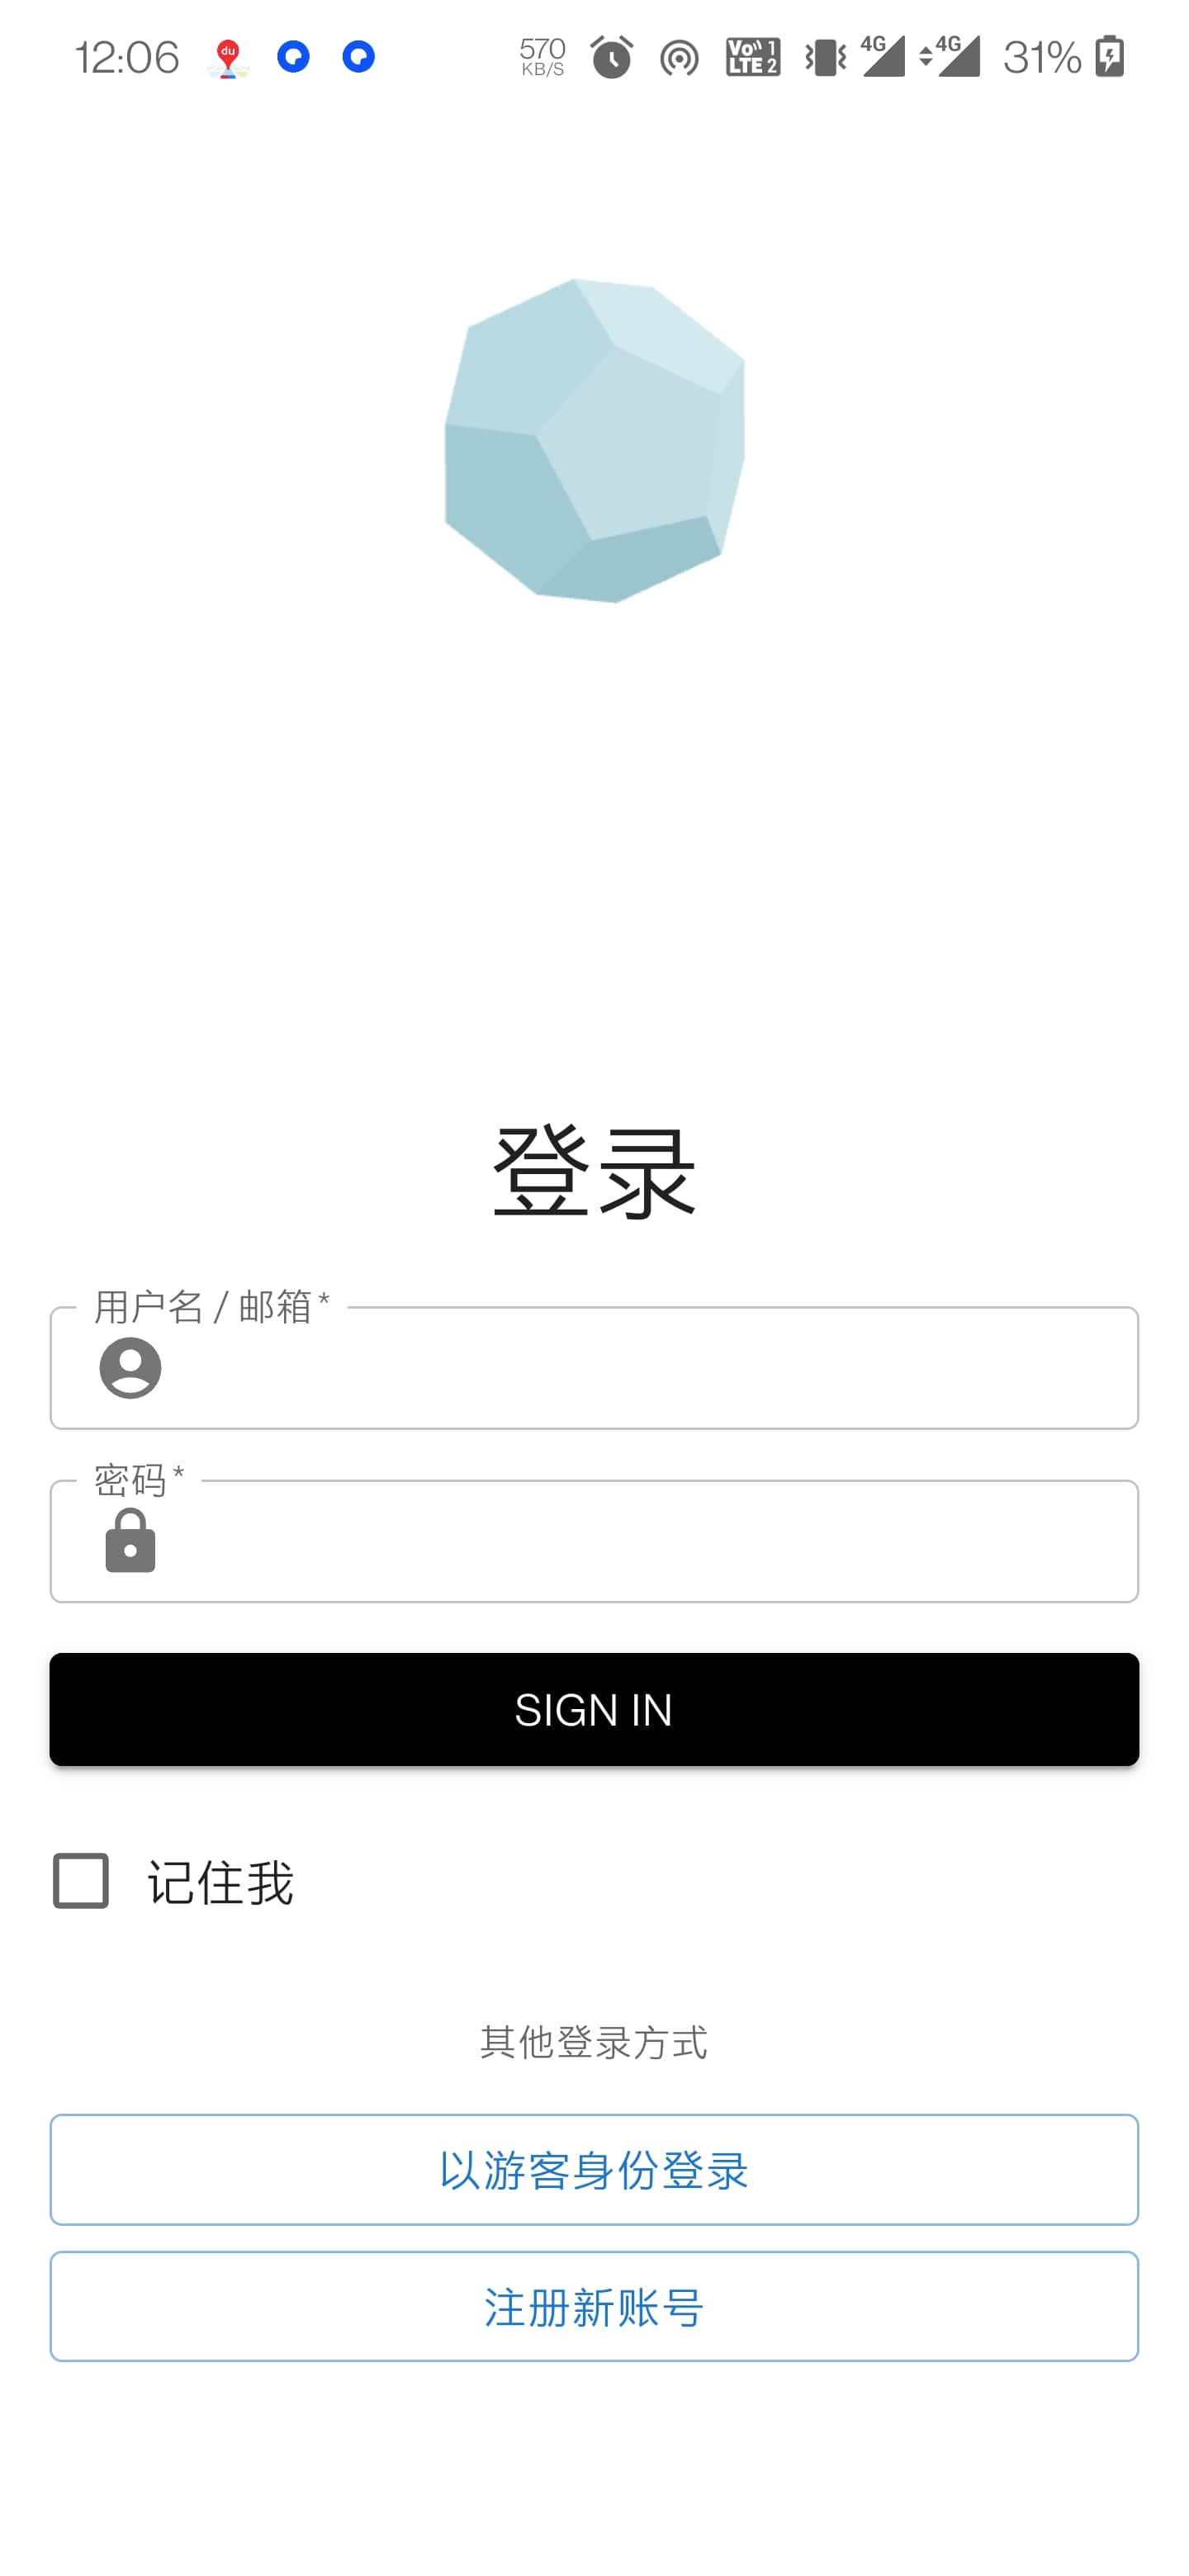
\includegraphics[width=4cm]{./figs/login.jpg}};
      \draw [Circle-] (-1.75,-0.3) -- (-3,-0.3) node [left] {输入用户名或邮箱};
      \draw [Circle-] (-1.75,-0.8) -- (-3,-0.8) node [left] {输入密码};
      \draw [Circle-] (-1.75,-1.5) -- (-3,-1.5) node [left] {点击提交表单};
      \draw [Circle-] (-1.75,-2.1) -- (-3,-2.1) node [left] {localstroge 登录记录};
      \draw [Circle-] (1.75,-2.1) -- (3,-2.1) node [right] {重制密码};
      \draw [Circle-] (-1.75,-2.9) -- (-3,-2.9) node [left] {跳过登录,进入系统};
      \draw [Circle-] (-1.75,-3.3) -- (-3,-3.3) node [left] {进入注册界面};
    \end{scope}
  \end{tikzpicture}
  \caption{登录界面}
  \label{fig:登录界面}
\end{figure}

注册界面提供新用户注册功能,注册逻辑与常用手机 app 相同,必填数据选以 * 标注,注册界面如图\ref{fig:注册界面}所示:

\begin{figure}[H]
  \small
  \centering
  \begin{tikzpicture}[font=\footnotesize]
    \begin{scope}[xshift=0cm]
      \node () at (-7,0) {};
      \node () at (7,0) {};
      \node [draw=black!60] (fig) at (0,0) {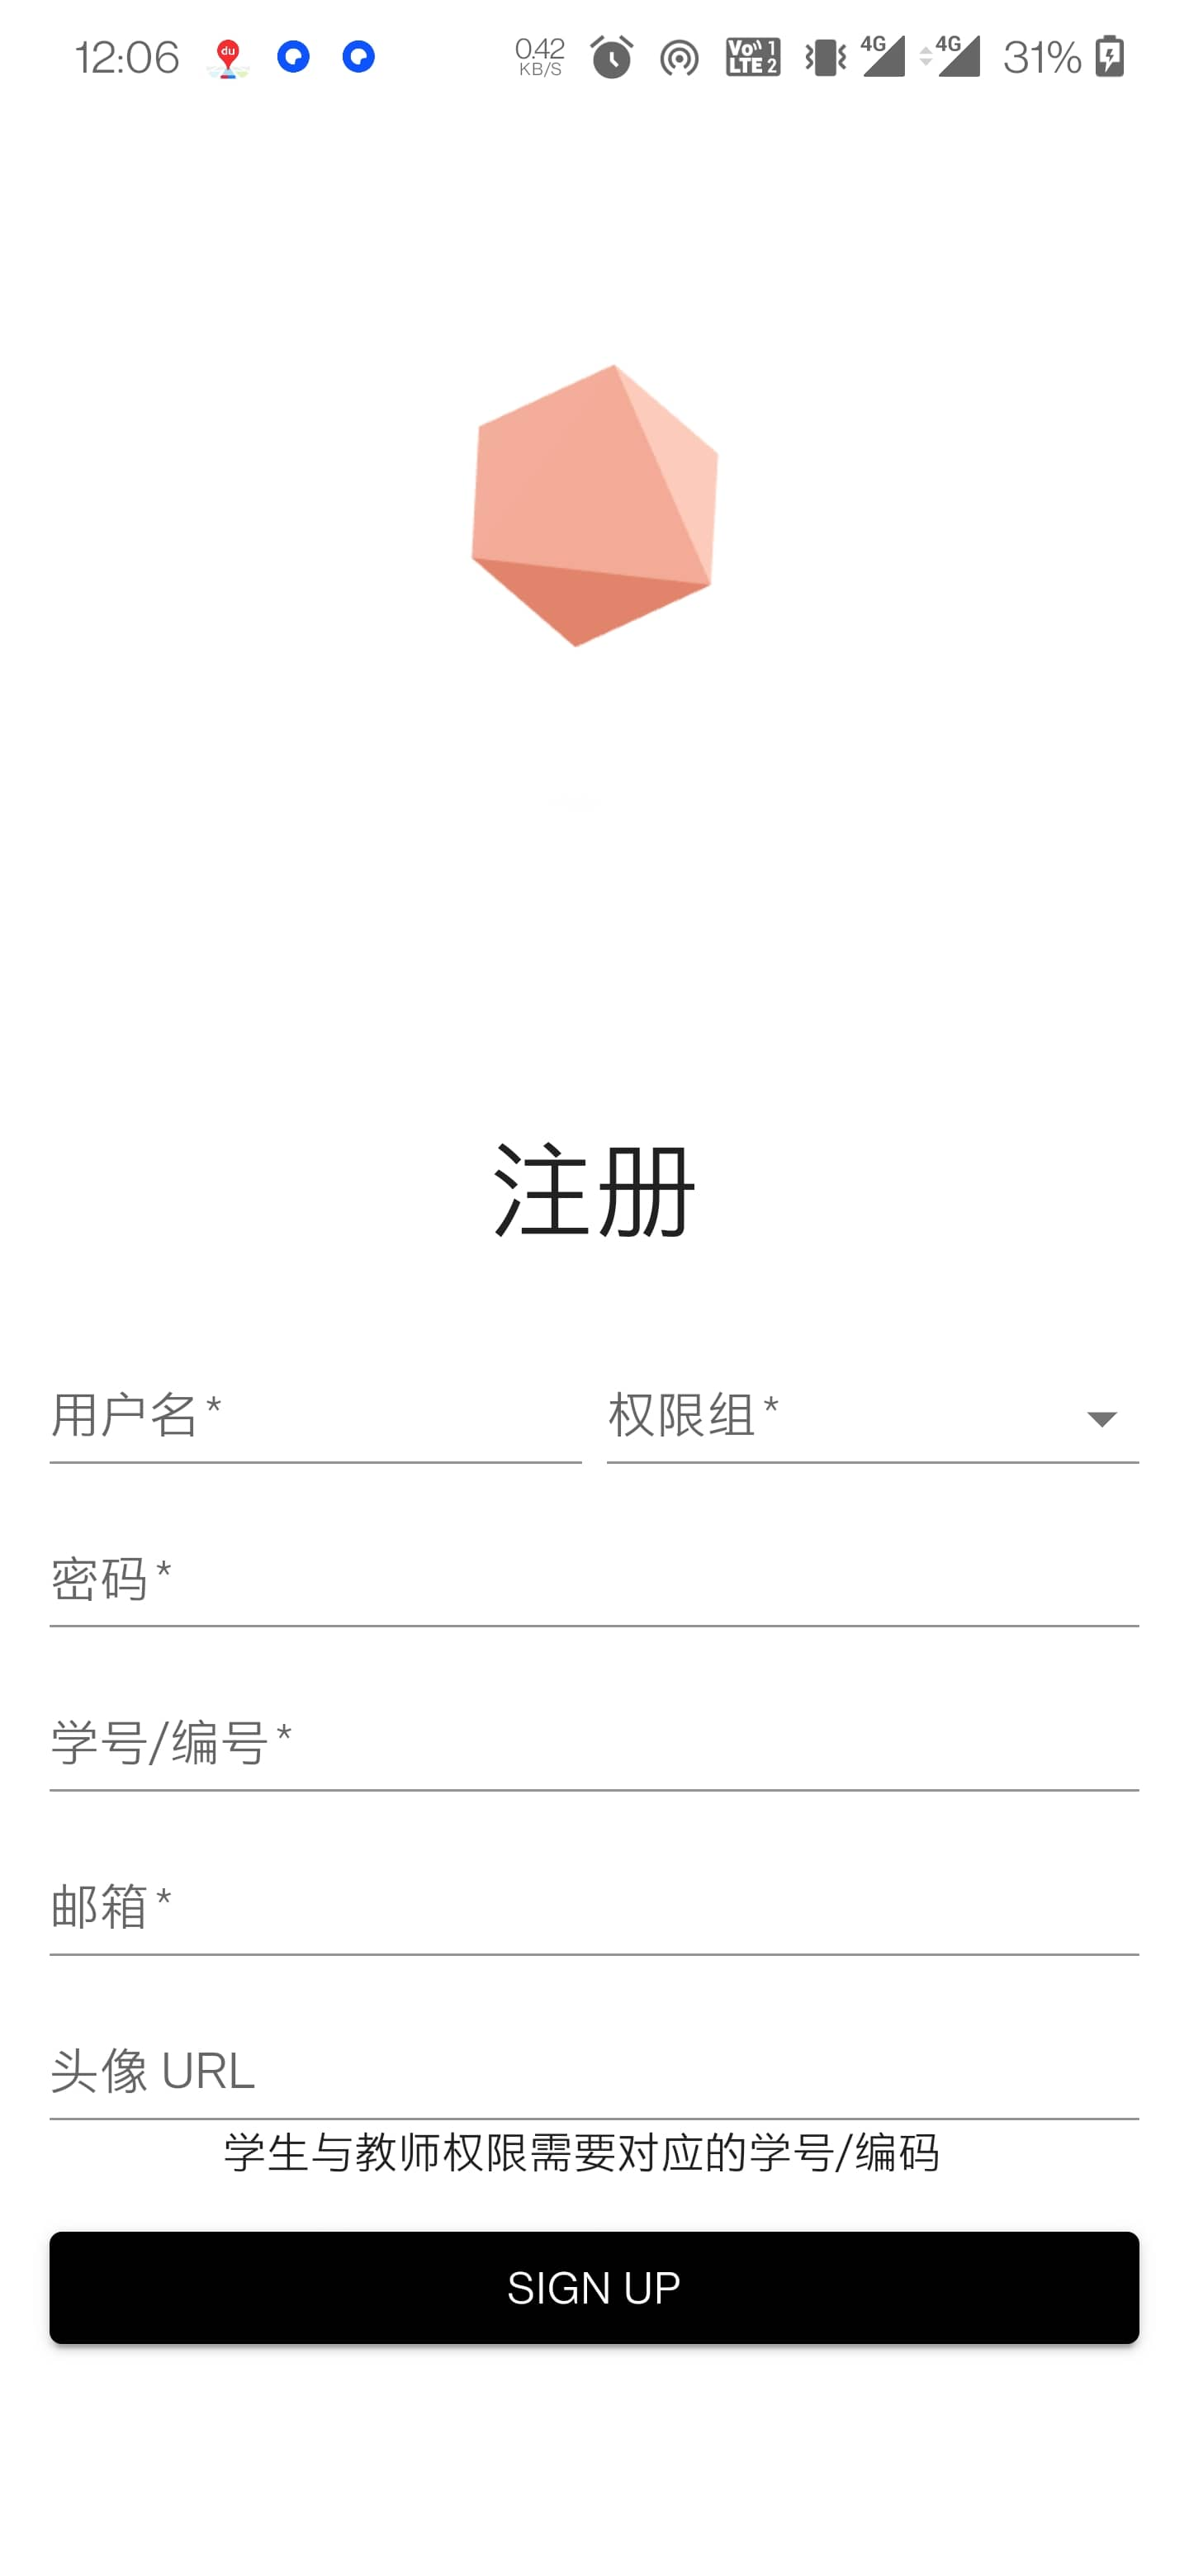
\includegraphics[width=4cm]{./figs/registry.jpg}};
      \draw [Circle-] (-1.75,0) -- (-3,0) node [left] {必填数据段,* 标识};
      \draw [Circle-] (-1.75,-0.9) -- (-3,-0.9) node [left] {可选数据段};
      \draw [Circle-] (-1.75,-2.8) -- (-3,-2.8) node [left] {注册按钮,提交表单};
    \end{scope}
  \end{tikzpicture}
  \caption{注册界面}
  \label{fig:注册界面}
\end{figure}

我的界面向用户展示个人信息,同时提供一些快捷服务,用户可以在此修改个人信息,我的界面如图\ref{fig:我的界面}所示:

\begin{figure}[H]
  \small
  \centering
  \begin{tikzpicture}[font=\footnotesize]
    \begin{scope}[xshift=0cm]
      \node () at (-7,0) {};
      \node () at (7,0) {};
      \node [draw=black!60] (fig) at (0,0) {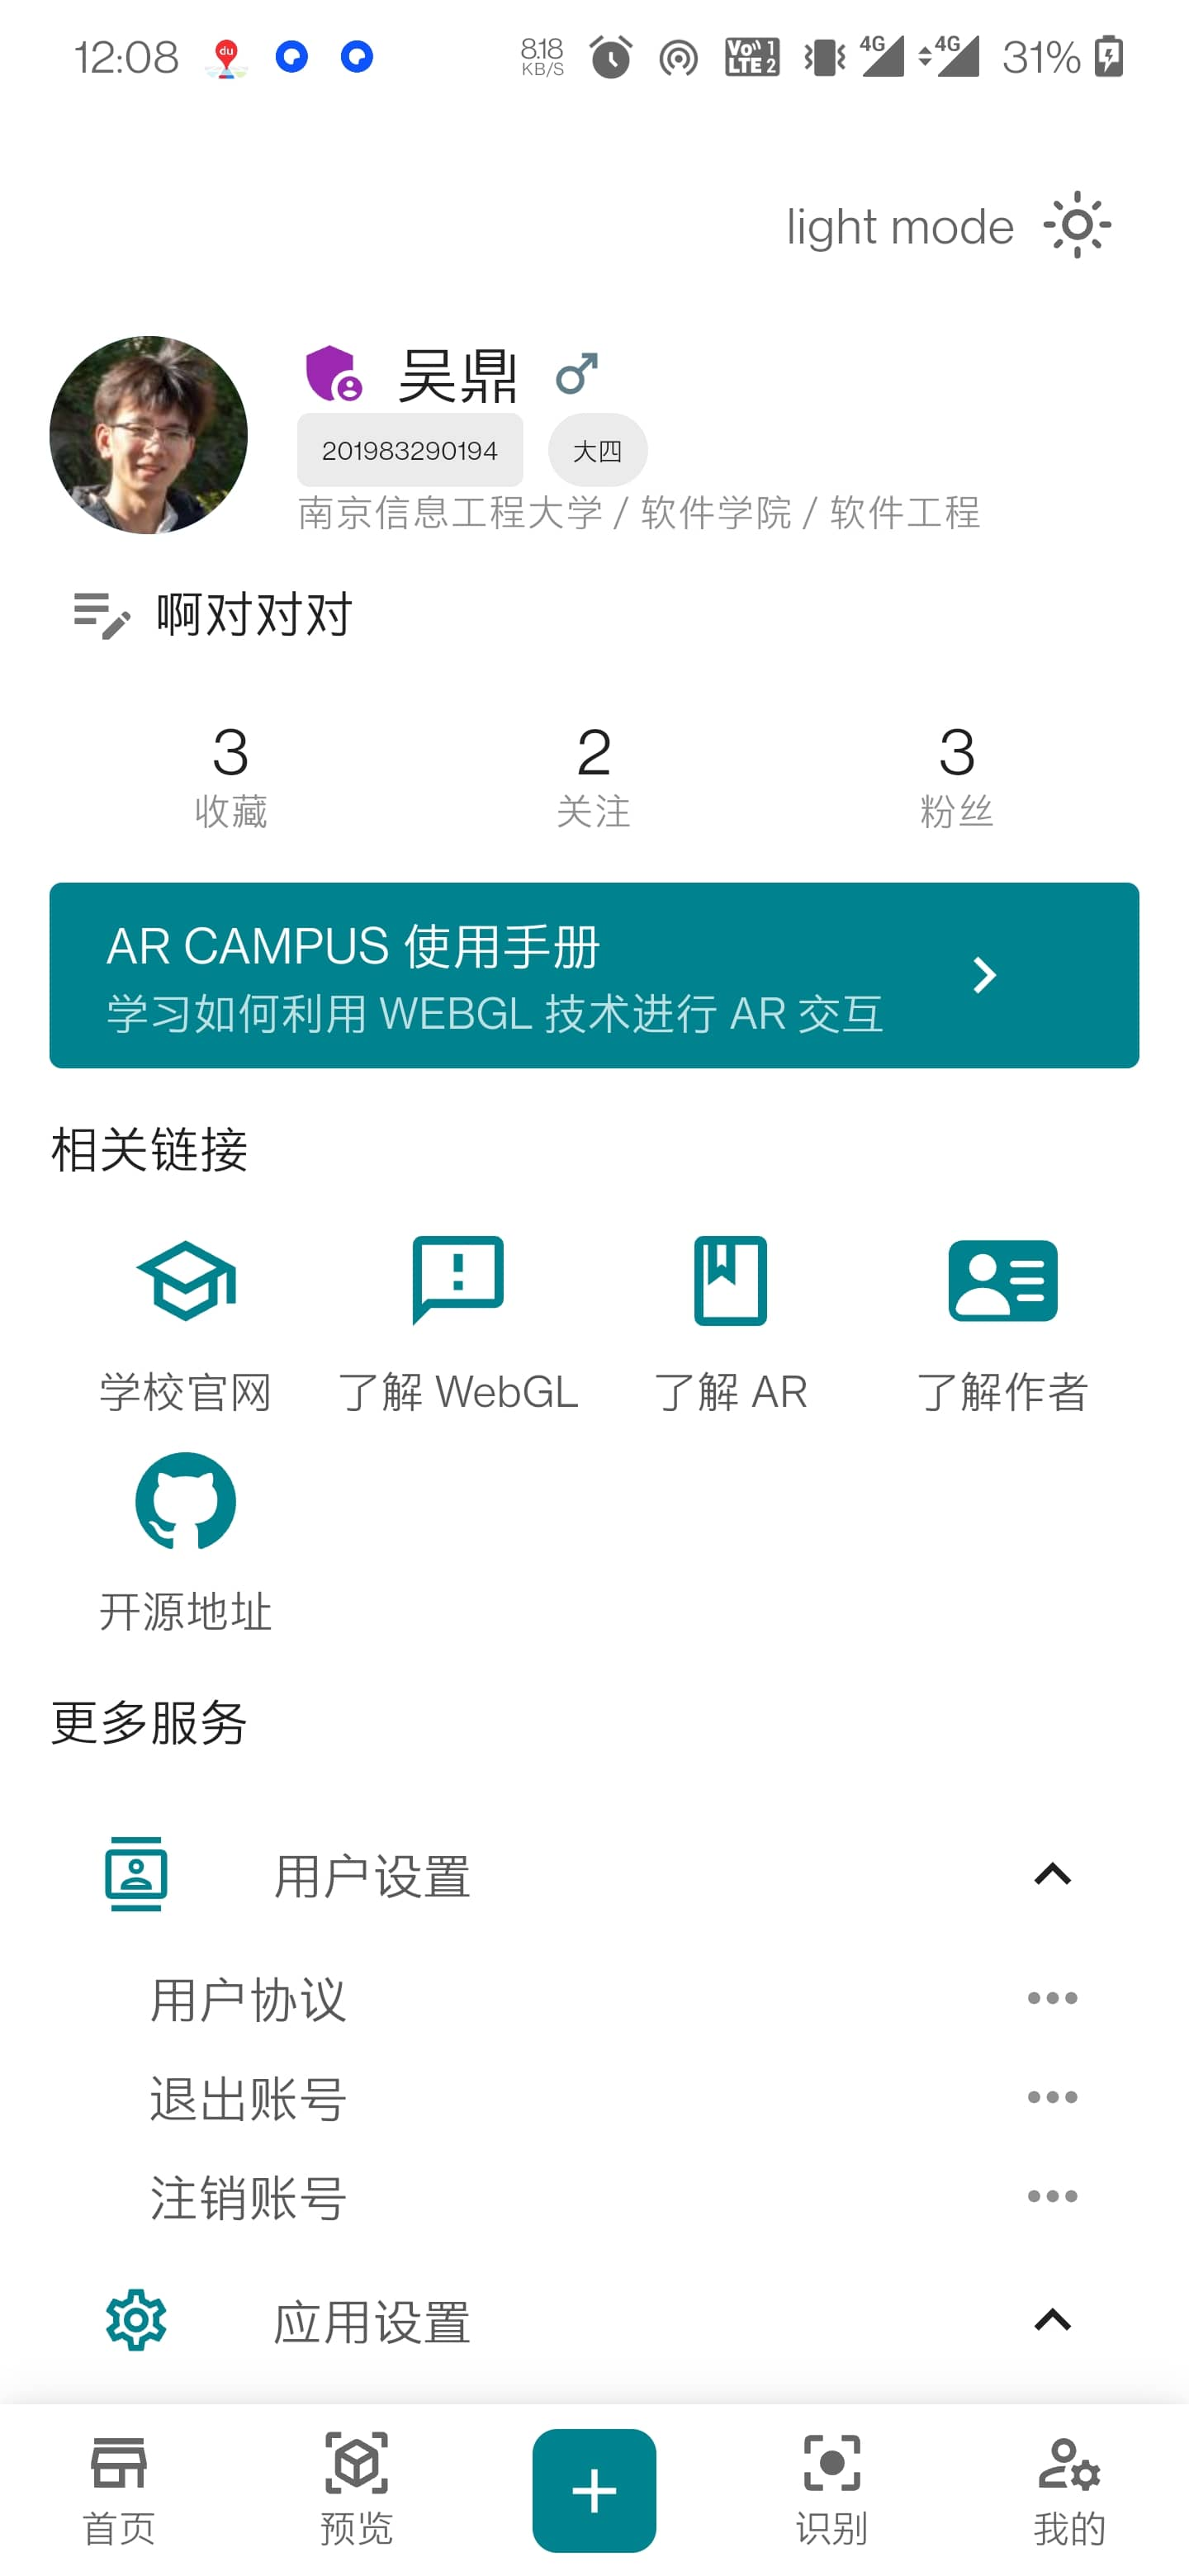
\includegraphics[width=4cm]{./figs/my.jpg}};
      \draw [Circle-] (1.75,3.6) -- (3,3.6) node [right] {切换主题,设置主题色};
      \draw [Circle-] (-1.75,2.88) -- (-3,2.88) node [left] {用户主要信息};
      \draw [Circle-] (-1.75,2.25) -- (-3,2.25) node [left] {修改签名};
      \draw [Circle-] (0.25,1.75) -- (3,1.75) node [right] {社区信息,点击可查看列表};
      \draw [Circle-] (1.75,1) -- (3,1) node [right] {活动面板,展示主要活动或提示};
      \draw [Circle-] (-1.75,0) -- (-3,0) node [left] {一些服务的快捷链接};
      \draw [Circle-] (-1.75,-1.25) -- (-3,-1.25) node [left] {设置,可展开};
      \draw [Circle-] (-1.75,-4) -- (-3,-4) node [left] {其他模块链接};
    \end{scope}
  \end{tikzpicture}
  \caption{我的界面}
  \label{fig:我的界面}
\end{figure}

\subsubsection{数据推送}

数据推送模块包含首页界面。

用户进入首页可根据需求选择分区: ``为你推荐'', ``最新更新'', ``我的关注''。后端将根据用户选择采用对应算法传输可用数据到前端。同时用户也可手动搜索内容。

主页瀑布流中将显示各个模型的简要信息,包括预览图片,名称,作者等,用户点击对应卡片即可预览 3D 模型。``主页''界面如图\ref{fig:主页界面}所示:

\begin{figure}[H]
  \small
  \centering
  \begin{tikzpicture}[font=\footnotesize]
    \begin{scope}[xshift=0cm]
      \node () at (-7,0) {};
      \node () at (7,0) {};
      \node [draw=black!60] (fig) at (0,0) {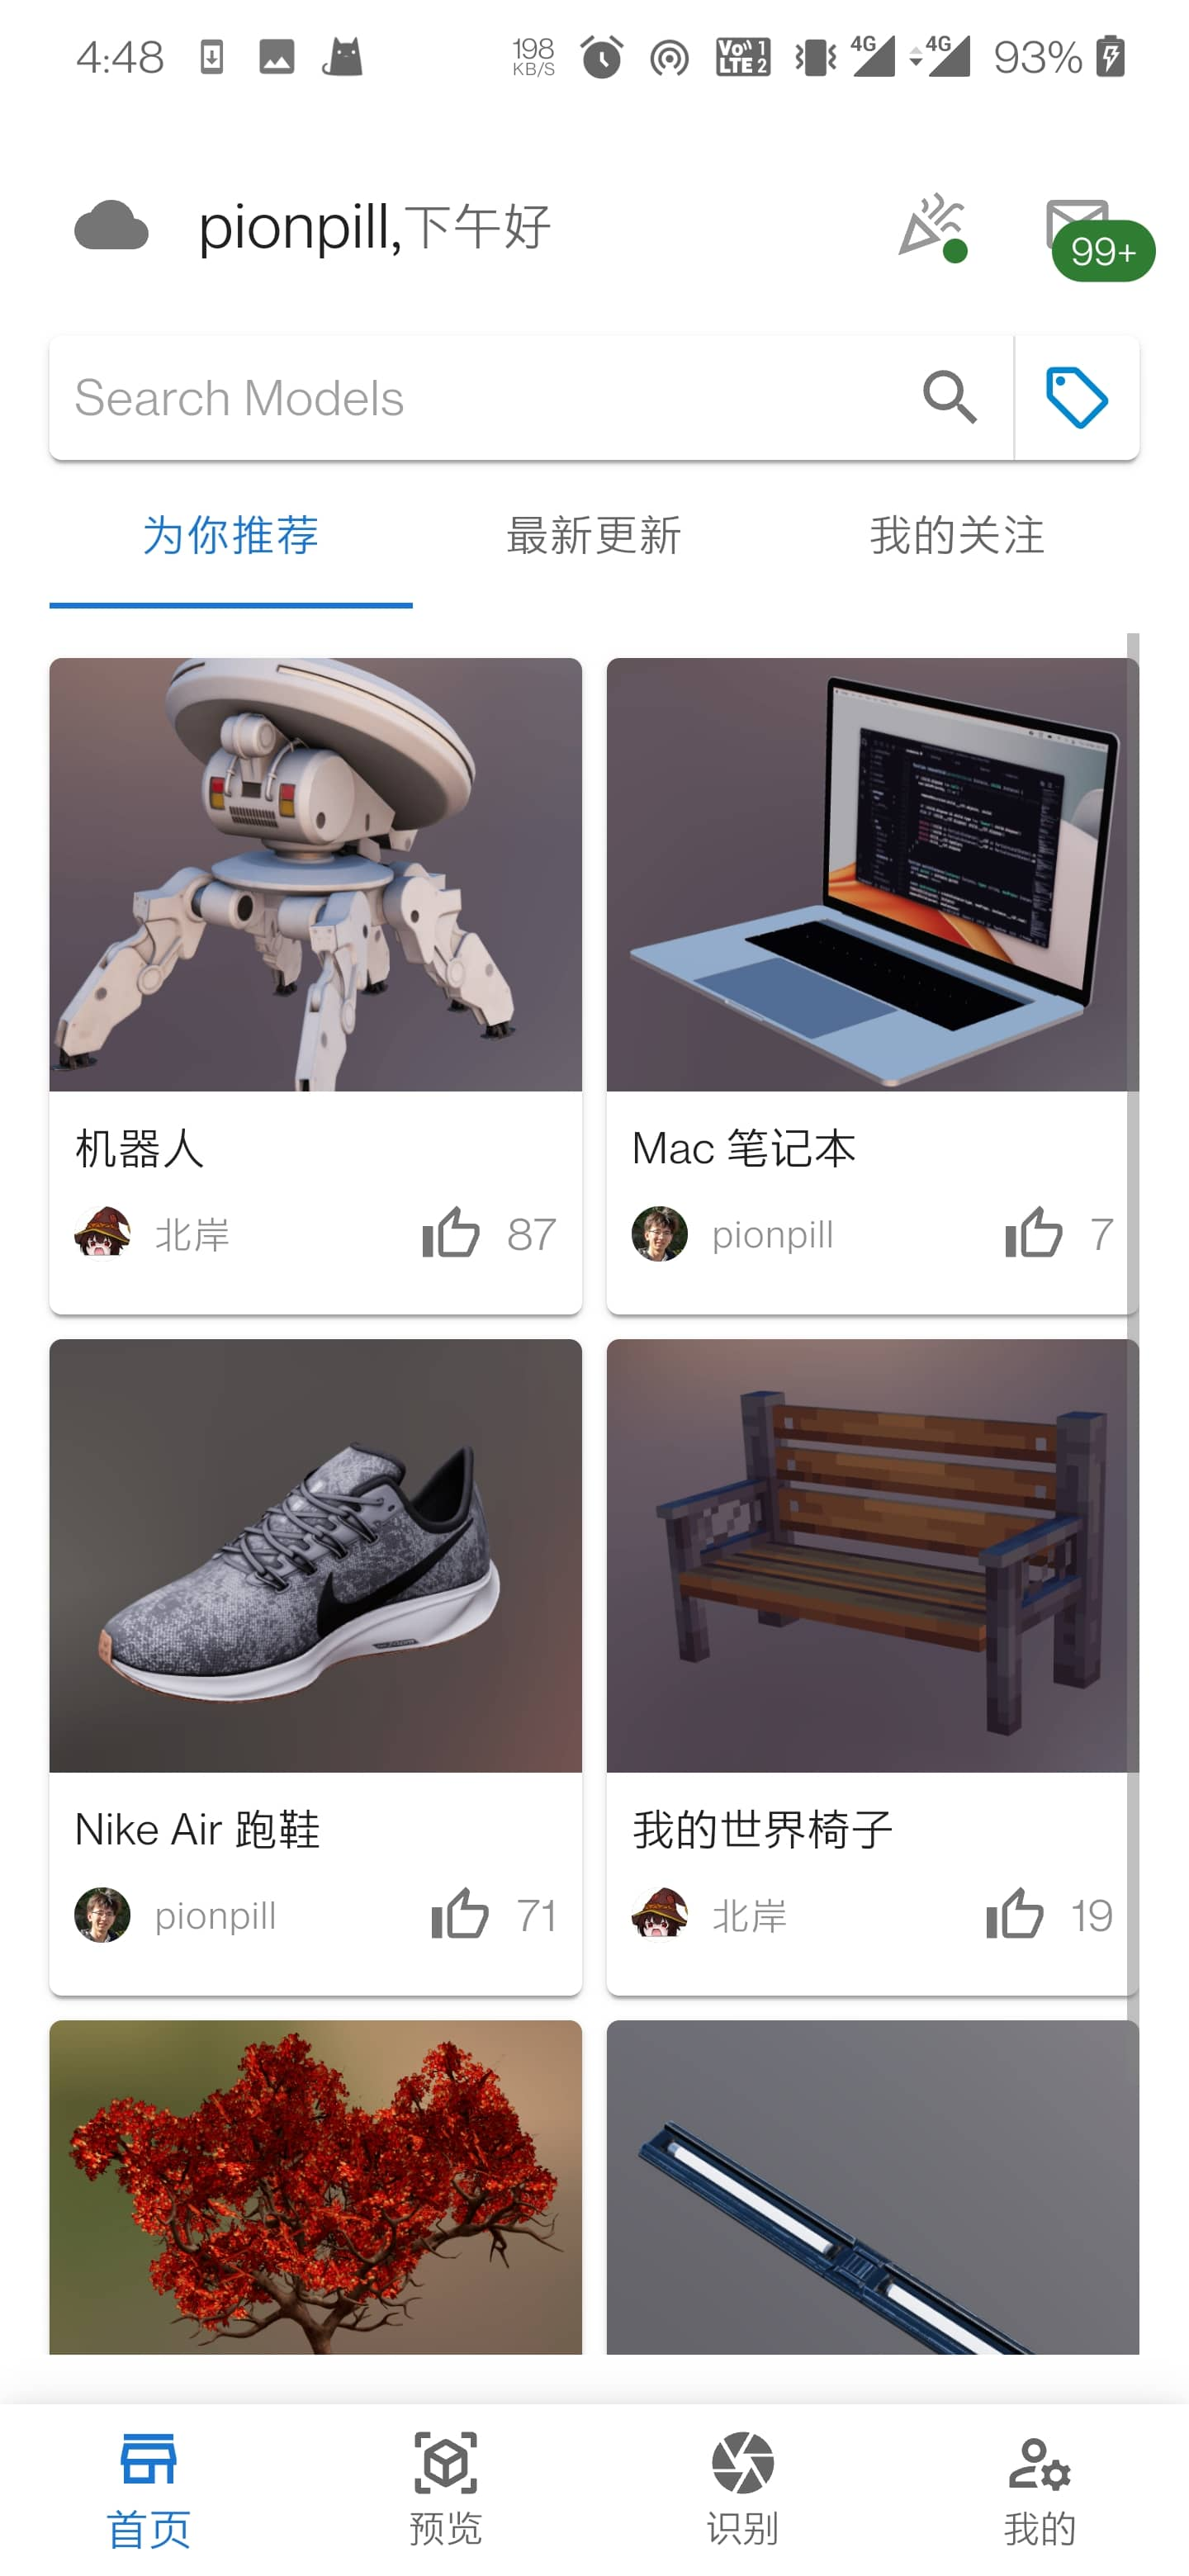
\includegraphics[width=4cm]{./figs/home.jpg}};
      \draw [Circle-] (1.1,3.5) |- (3,3.8) node [right] {系统的一些更新提示};
      \draw [Circle-] (1.75,3.5) -- (3,3.5) node [right] {预留的邮箱功能,可接入邮箱系统};
      \draw [Circle-] (-1.75,3.5) -- (-3,3.5) node [left] {接入高德天气服务};
      \draw [Circle-] (-1.75,2.95) -- (-3,2.95) node [left] {搜索框};
      \draw [Circle-] (-1.75,2.5) -- (-3,2.5) node [left] {分区类型};
      \draw [Circle-] (-0.5,1) -- (-3,1) node [left] {模型卡,点击预览};
      \draw [Circle-] (0.75,1.75) -- (3,1.75) node [right] {模型封面};
      \draw [Circle-] (1,0.5) -- (3,0.5) node [right] {模型名称};
      \draw [Circle-] (-1.75,0.2) -- (-3,0.2) node [left] {作者};
      \draw [Circle-] (1.5,0.2) -- (3,0.2) node [right] {点赞数据};
      \draw [Circle-] (-1.75,-4) -- (-3,-4) node [left] {其他模块链接};
    \end{scope}
  \end{tikzpicture}
  \caption{主页界面}
  \label{fig:主页界面}
\end{figure}

\subsection{核心功能实现}
\subsubsection{WebGL 模块}

WebGL 模块包含模型预览界面。

用户进入模型预览界面后,系统将搭建场景,显示模型信息,请求模型信息数据:
\begin{itemize}
  \item 搭建场景: 系统通过模型 id 查模型表和模型控制表,获取模型 url 和相关配置信息。此时系统将显示场景。
  \item 请求模型: 系统获取模型 url 后异步请求模型数据,继而在界面上显示。
  \item 模型信息: 系统向后端请求模型的文本,点赞,作者等信息。
\end{itemize}

其中搭建场景,显示模型信息的功能同步进行,模型数据异步请求。

预览界面将模型信息分为简要信息与详细信息,简要信息仅以浮动卡片形式显现,用户可隐藏相关信息。详细信息则无法隐藏。用户在移动设备上可通过触摸移动位置,双指缩放模型大小,也可以通过控制板调整环境信息,例如背景贴图,背景模糊程度。模型预览界面如图\ref{fig:模型预览界面}所示:

\begin{figure}[H]
  \small
  \centering
  \begin{tikzpicture}[font=\footnotesize]
    \node () at (-7,0) {};
    \node () at (7,0) {};
    \begin{scope}[xshift=-2.25cm]
      \node [draw=black!60] (fig) at (0,0) {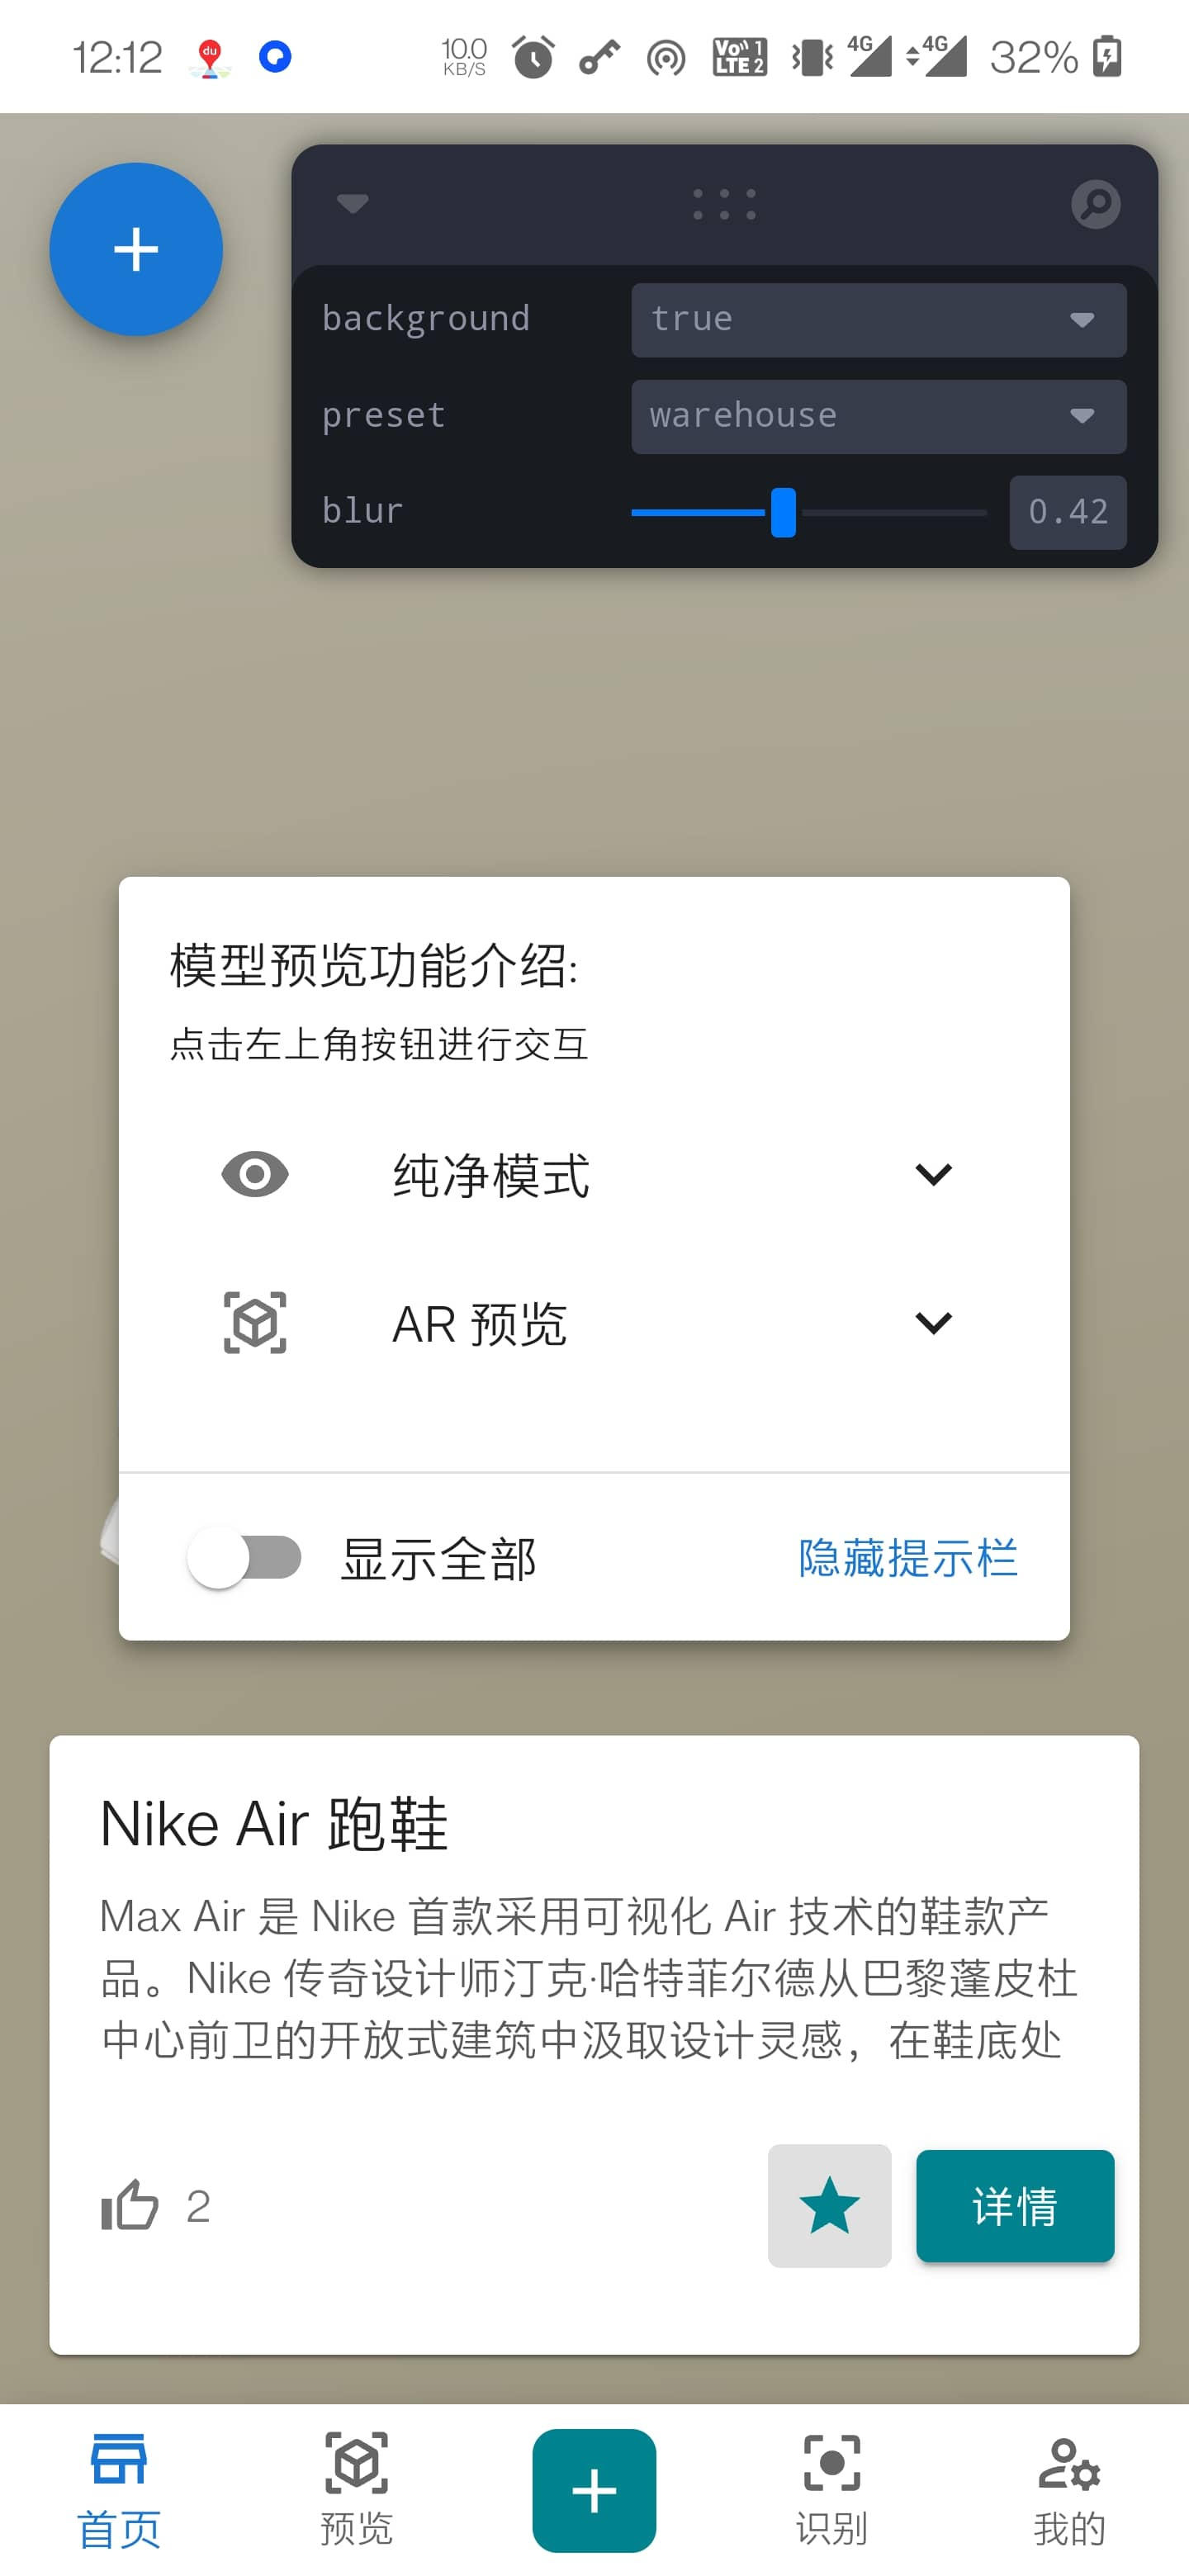
\includegraphics[width=4cm]{./figs/preview.jpg}};
      \draw [Circle-] (-0.5,3.75) -- (-3,3.75) node [left] {控制板};
      \draw [Circle-] (-1.75,3.5) -- (-3,3.5) node [left] {扩展功能按钮};
      \draw [Circle-] (-1.75,2.5) -- (-3,2.5) node [left] {场景背景};
      \draw [Circle-] (-1.5,0.2) -- (-3,0.2) node [left] {操作说明};
      \draw [Circle-] (-1.5,-1) -- (-3,-1) node [left] {快捷功能按钮};
      \draw [Circle-] (-1.75,-1.8) -- (-3,-1.8) node [left] {模型名称};
      \draw [Circle-] (-1.75,-2.2) -- (-3,-2.2) node [left] {模型简介};
      \draw [Circle-] (-1,-2.5) -- (-3,-2.5) node [left] {简要信息卡};
      \draw [Circle-] (-1.75,-3.1) -- (-3,-3.1) node [left] {模型点赞数据};
      \draw [Circle-] (0.75,-3.1) |- (-3,-2.8) node [left] {用户收藏按钮};
      \draw [Circle-] (1.5,-3.1) |- (-3,-3.4) node [left] {切换到详细信息};
      \draw [Circle-] (-1.75,-4) -- (-3,-4) node [left] {其他模块链接};
    \end{scope}
    \begin{scope}[xshift=2.25cm]
      \node () at (-7,0) {};
      \node () at (7,0) {};
      \node [draw=black!60] (fig) at (0,0) {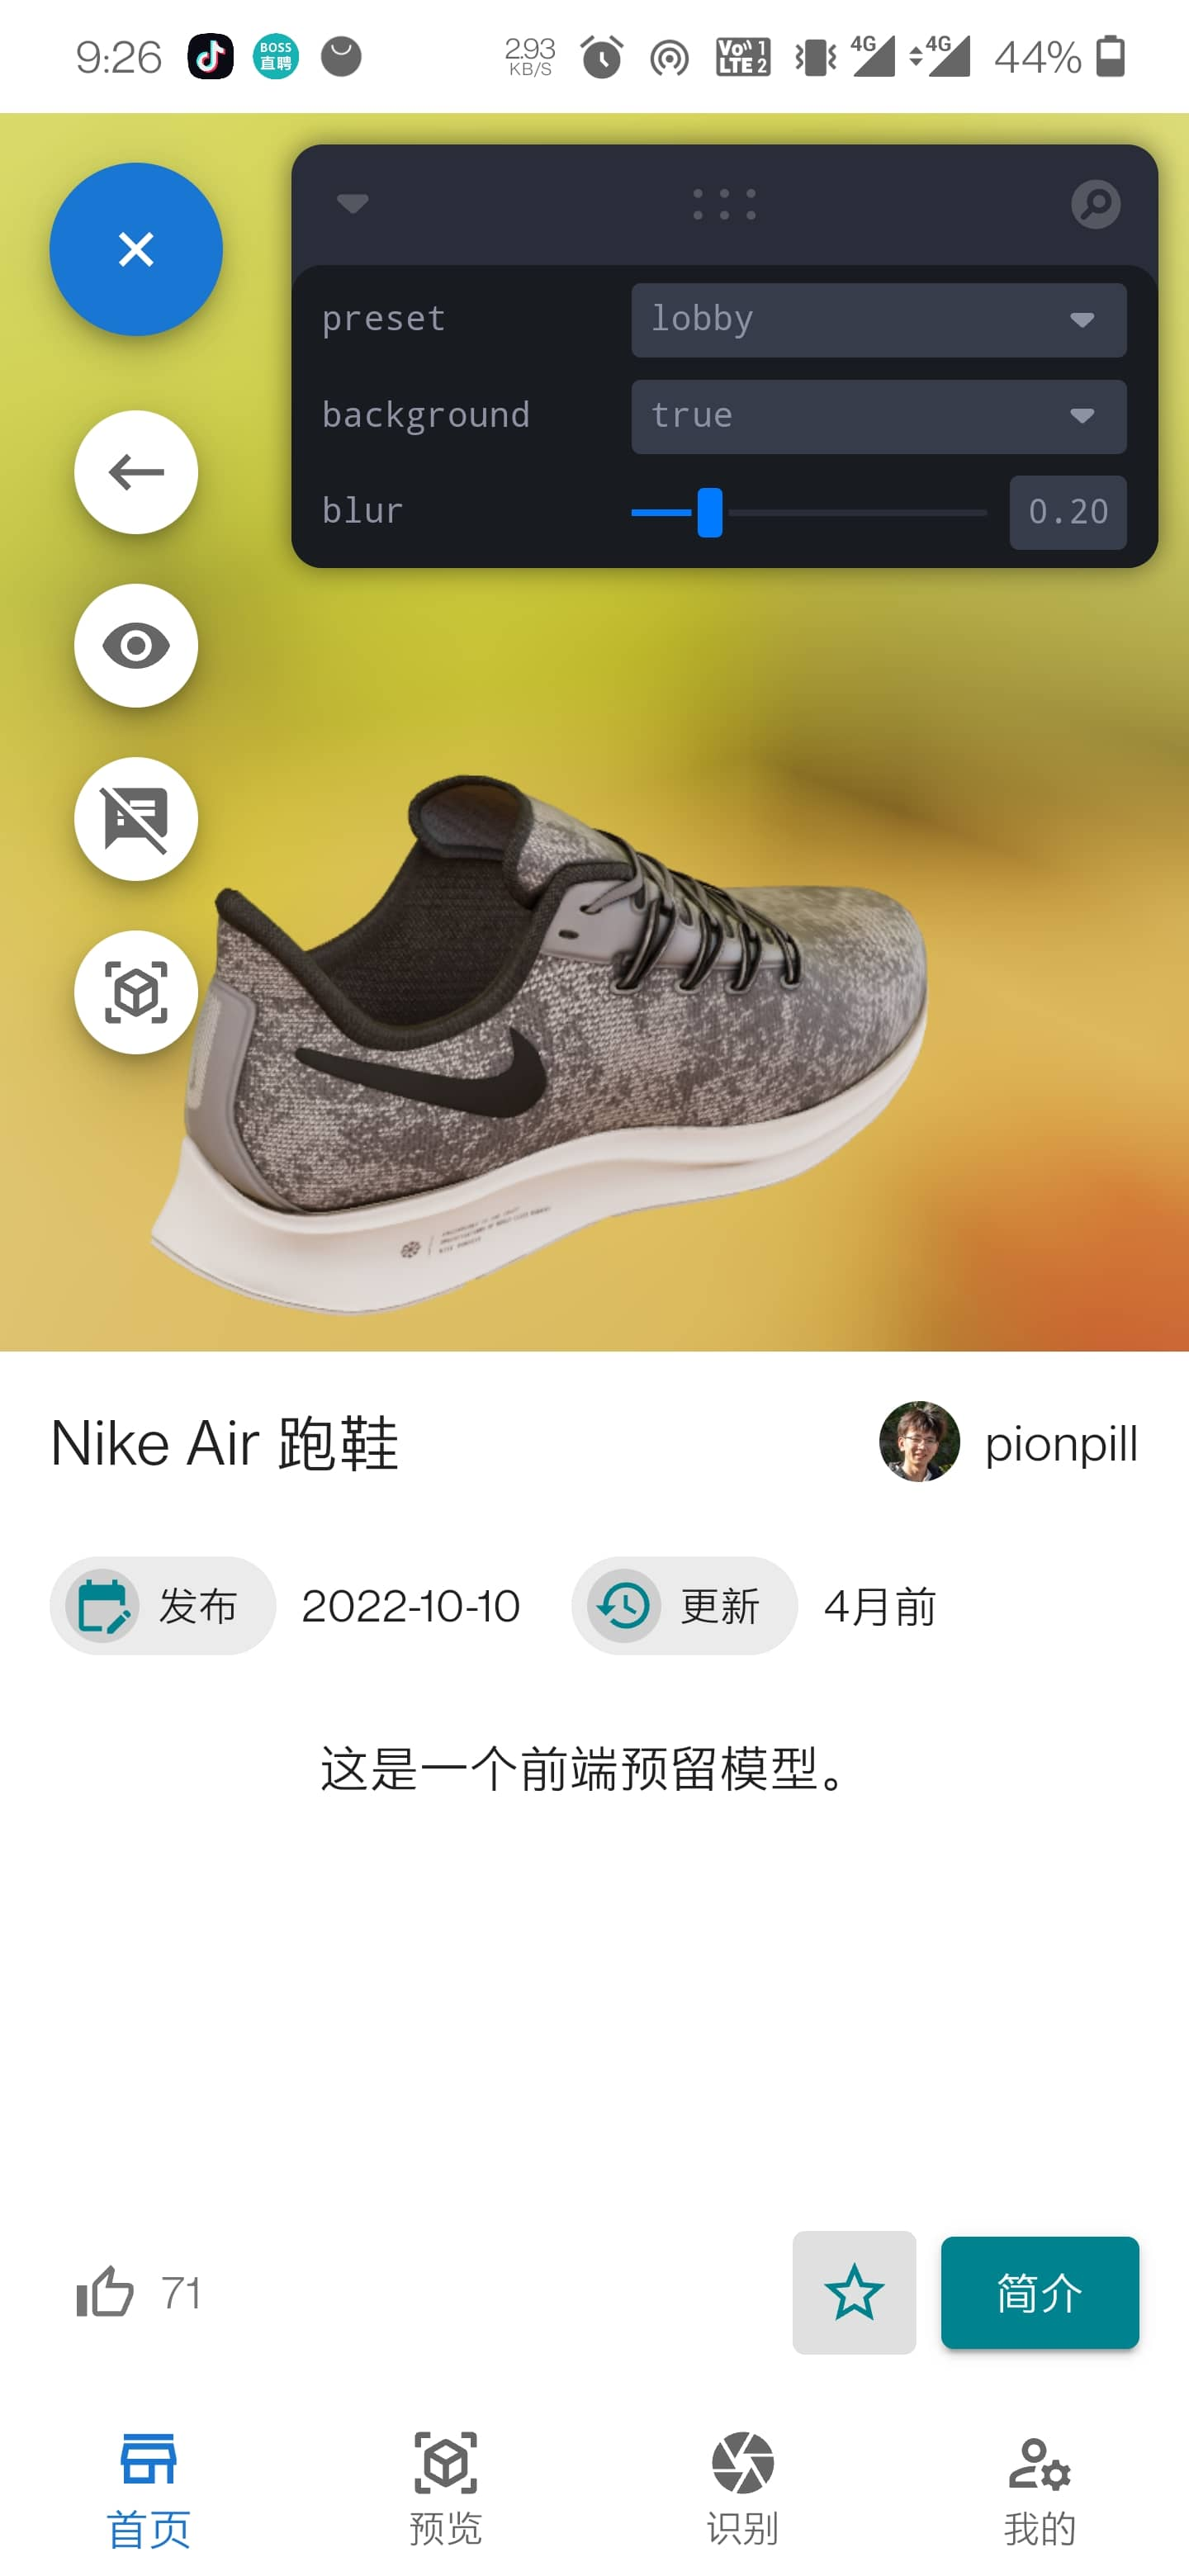
\includegraphics[width=4cm]{./figs/preview-2.jpg}};
      \draw [Circle-] (1.75,3.3) -- (3,3.3) node [right] {切换环境背景};
      \draw [Circle-] (1.75,2.9) -- (3,2.9) node [right] {切换是否显示背景};
      \draw [Circle-] (1.75,2.5) -- (3,2.5) node [right] {设置背景模糊程度};
      \draw [Circle-] (0,0.5) -- (3,0.5) node [right] {模型本体};
      \draw [Circle-] (2,-0.5) -- (3,-0.5) node [right] {作者信息};
      \draw [Circle-] (1.5,-1) -- (3,-1) node [right] {模型发布与更新信息};
      \draw [Circle-] (1.75,-1.8) -- (3,-1.8) node [right] {模型详细信息};
      \draw [Circle-] (1.75,-4) -- (3,-4) node [right] {其他模块链接};
      \draw [Circle-] (-1.4,2.2) -- (3,2.2) node [right] {开关非必要组件};
      \draw [Circle-] (-1.4,1.6) -- (3,1.6) node [right] {开关操作说明};
      \draw [Circle-] (-1.4,1) -- (3,1) node [right] {在 AR 模式中显示};
    \end{scope}
  \end{tikzpicture}
  \caption{模型预览界面}
  \label{fig:模型预览界面}
\end{figure}

\subsubsection{AR 模块}

AR 模块包括 AR 预览与 AR 识别界面。

进入 AR 模式将提醒用户需要的设备条件,如果用户的设备不满足任意条件,AR 按钮将显示 AR unsupported。设备需要满足的条件如下:
\begin{itemize}
  \item 摄像头: 浏览器需要获取摄像头权限, 确保访问的是 https 协议网站,或者手动调整浏览器信任对应网站。否则浏览器无法获得摄像头权限。
  \item AR 服务: 安卓智能机需开启 AR 服务,请在 google play 安装 “面向 AR 的Google Play 服务” 插件。苹果设备开启 ARKit 服务。
  \item 浏览器: 尽量使用 chrome 浏览器,AR 功能至少需要 chrome 80+ 版本。安卓设备尽量保持在系统 11+ 版本。
  \item 网络环境: 出于优化考虑,系统不会一次推送所有数据,AR 部分功能需要实时获取网络资源。
\end{itemize}

AR 提示界面如图\ref{fig:AR提示界面}所示:

\begin{figure}[H]
  \small
  \centering
  \begin{tikzpicture}[font=\footnotesize]
    \begin{scope}[xshift=0cm]
      \node () at (-7,0) {};
      \node () at (7,0) {};
      \node [draw=black!60] (fig) at (0,0) {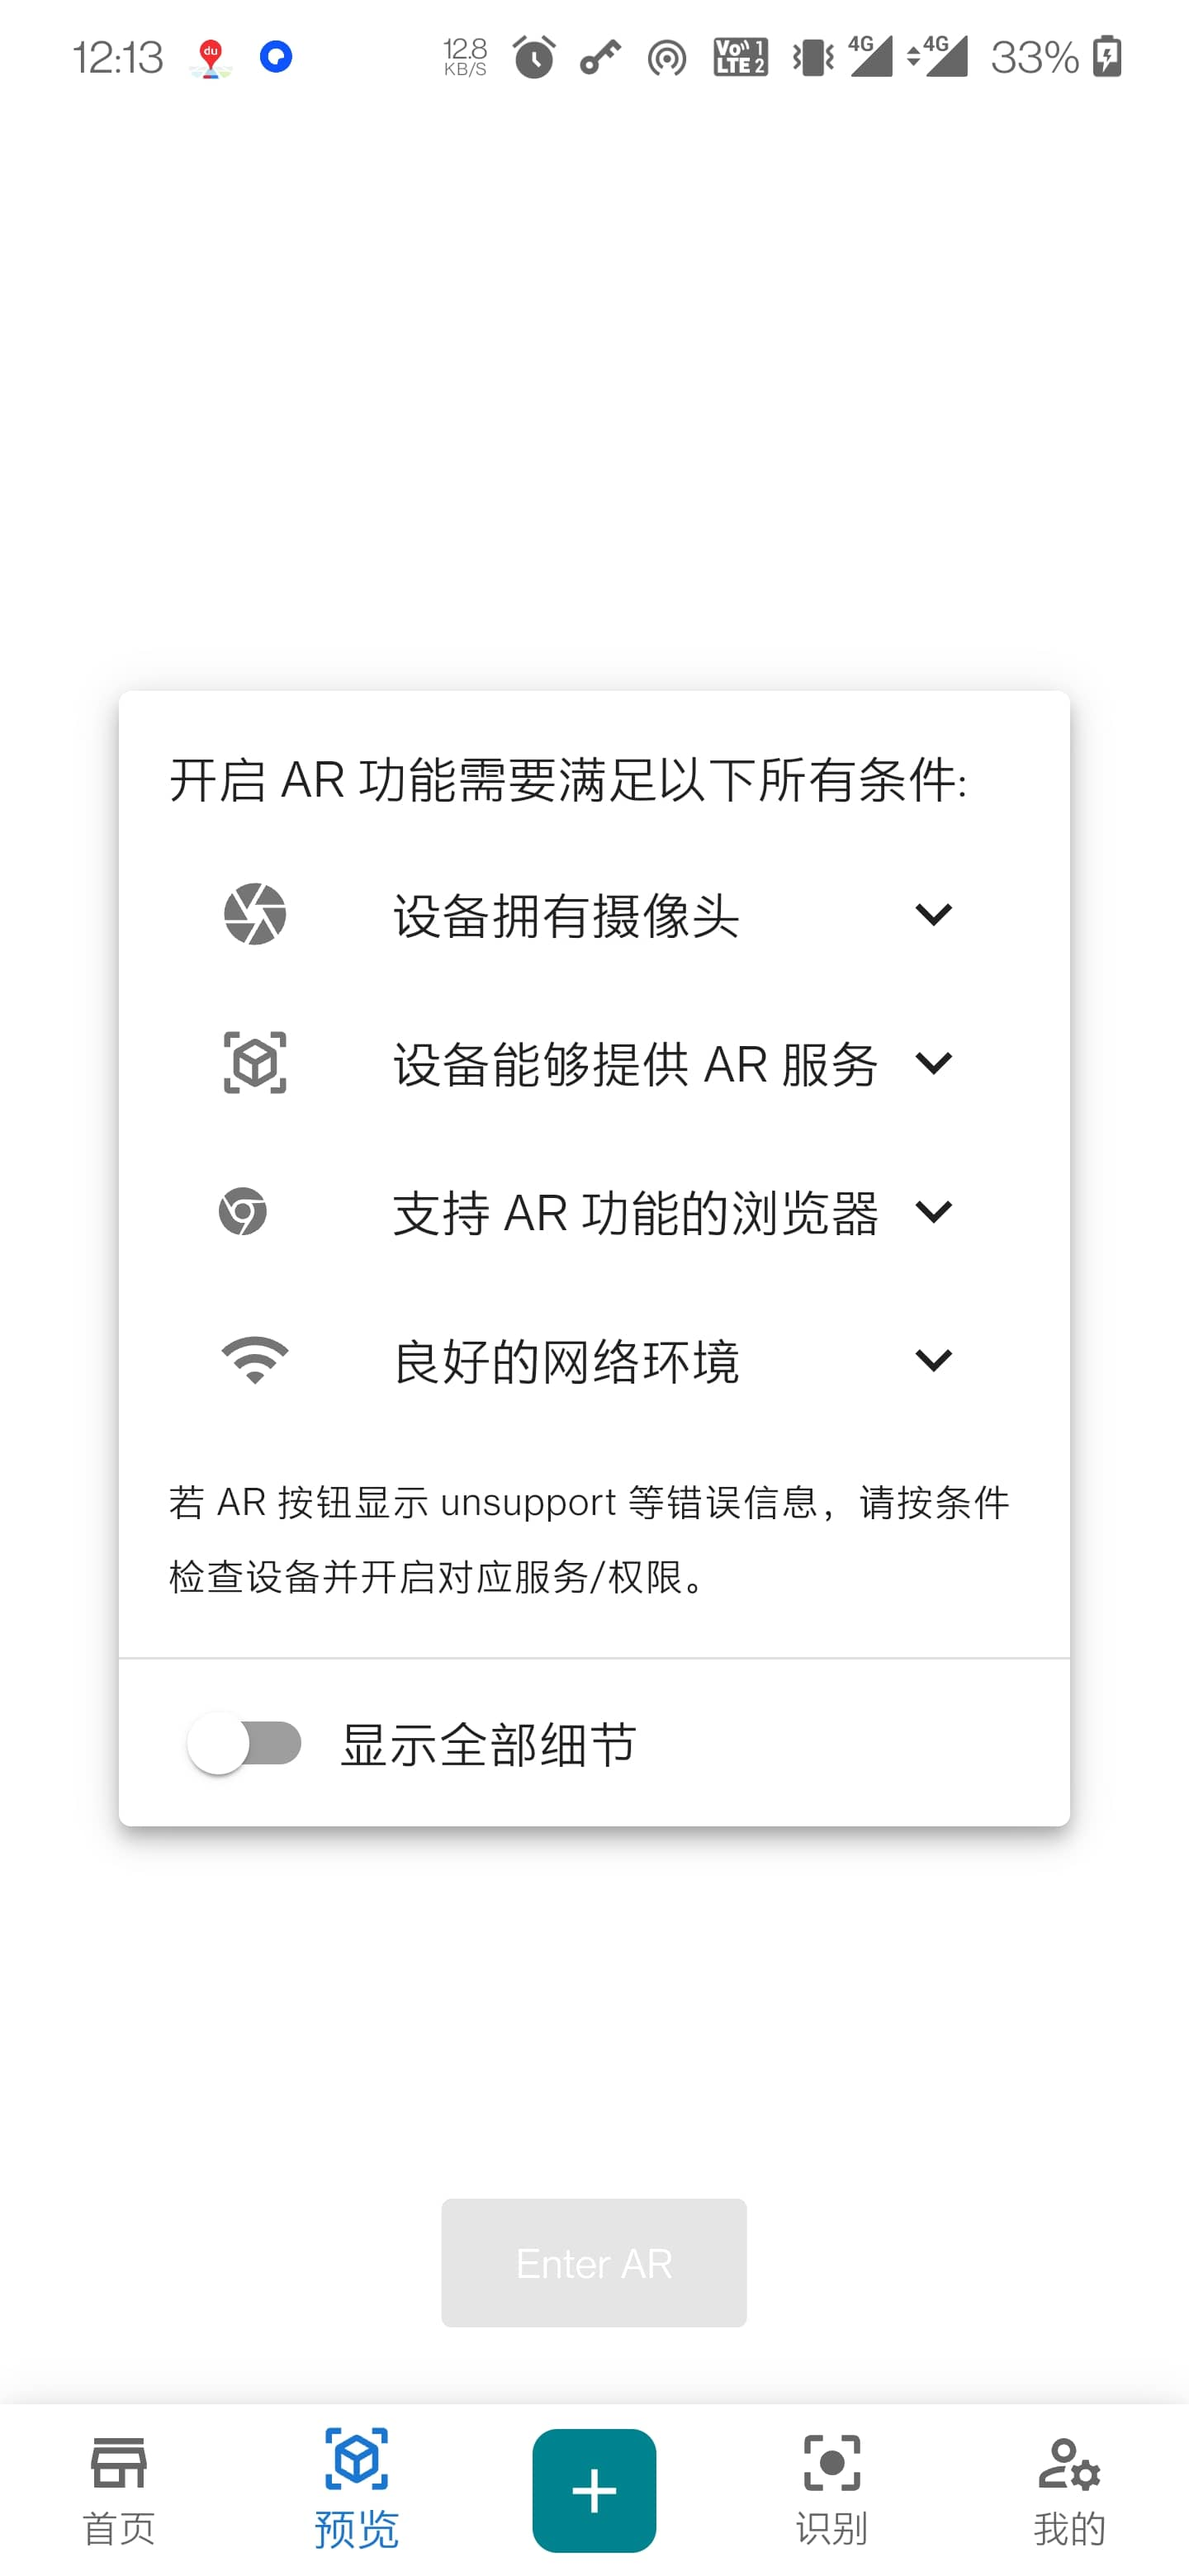
\includegraphics[width=4cm]{./figs/ar.jpg}};
      \draw [Circle-] (-0.5,1) -- (-3,1) node [left] {AR 提示信息};
      \draw [Circle-] (-1.5,-1.5) -- (-3,-1.5) node [left] {快捷操作按钮};
      \draw [Circle-] (-0.5,-3.25) -- (-3,-3.25) node [left] {AR 按钮};
      \draw [Circle-] (-1.75,-4) -- (-3,-4) node [left] {其他模块链接};
    \end{scope}
  \end{tikzpicture}
  \caption{AR提示界面}
  \label{fig:AR提示界面}
\end{figure}

进入 AR 预览界面后,系统会请求手机摄像头权限,用户确认之后,系统将实时获取显示影像,并将 3D 模式显示在界面中,用户可以通过控制板或手动调整操作模型。系统将实时计算模型所在位置,AR 预览界面如图\ref{fig:AR预览界面}所示:

\begin{figure}[H]
  \small
  \centering
  \begin{tikzpicture}[font=\footnotesize]
    \node () at (-7,0) {};
    \node () at (7,0) {};
    \begin{scope}[xshift=-2.25cm]
      \node [draw=black!60] (fig) at (0,0) {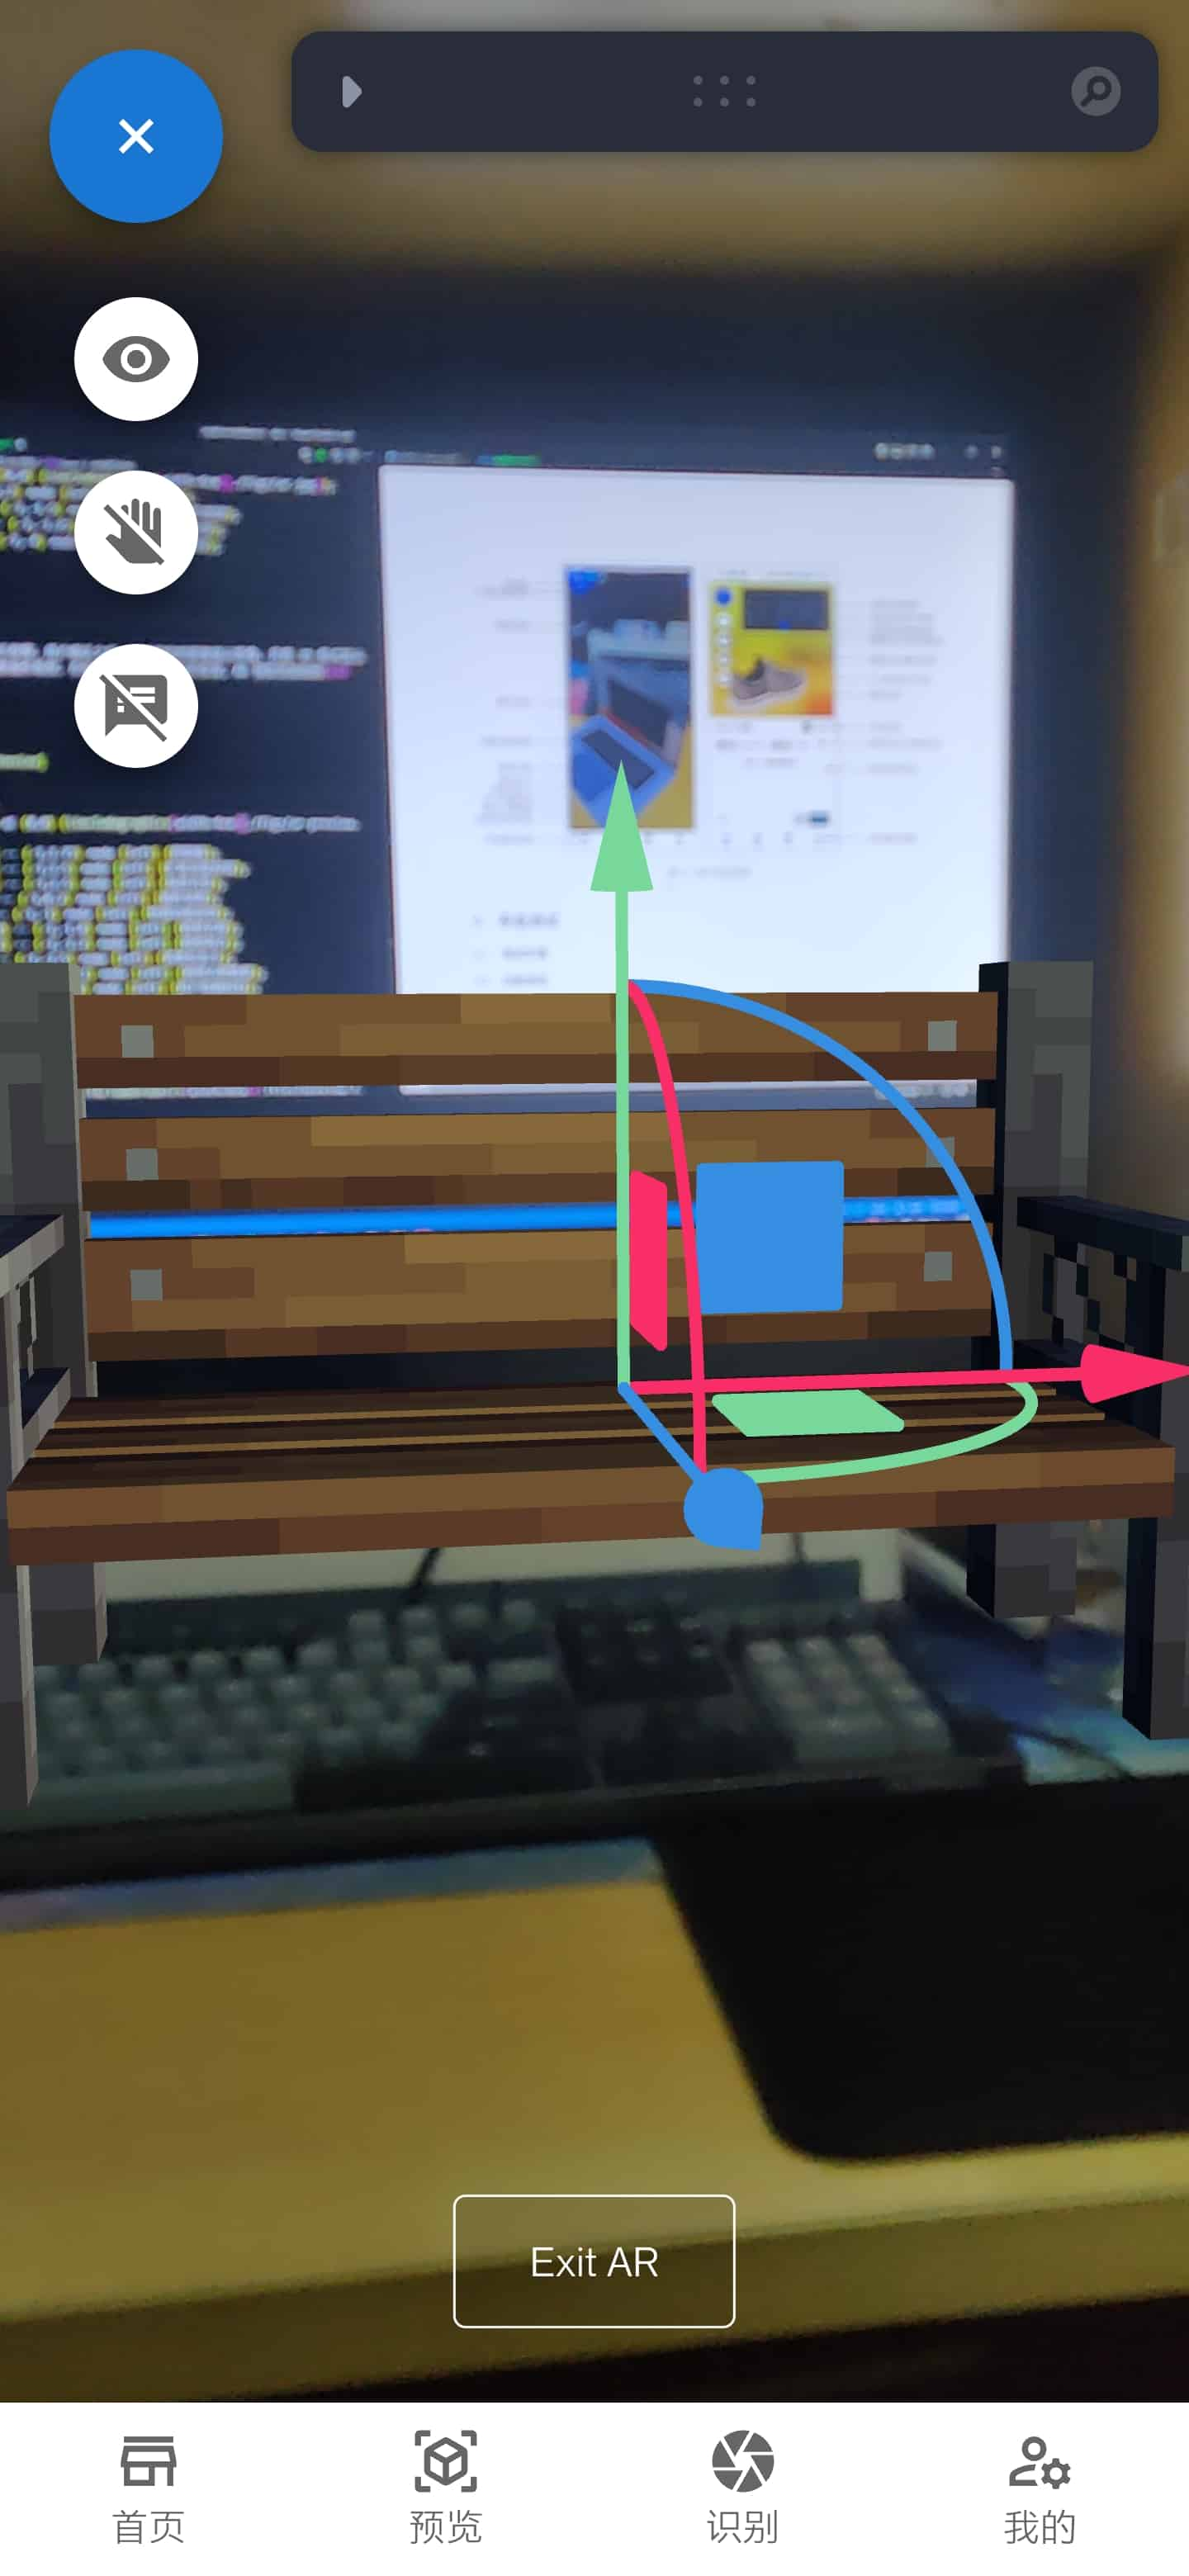
\includegraphics[width=4cm]{./figs/ar-preview.jpg}};
      \draw [Circle-] (-0.5,4) -- (-3,4) node [left] {控制板};
      \draw [Circle-] (-1.75,3.75) -- (-3,3.75) node [left] {扩展功能按钮};
      \draw [Circle-] (-1.75,3.1) -- (-3,3.1) node [left] {开关非必要组件};
      \draw [Circle-] (-1.75,2.5) -- (-3,2.5) node [left] {允许/禁止触控};
      \draw [Circle-] (-1.75,1.9) -- (-3,1.9) node [left] {开关操作说明};
      \draw [Circle-] (-1.5,0) -- (-3,0) node [left] {模型本体};
      \draw [Circle-] (0.5,-0.5) -- (-3,-0.5) node [left] {触摸操作轴};
      \draw [Circle-] (-1.5,-2) -- (-3,-2) node [left] {现实场景};
      \draw [Circle-] (-0.25,-3.25) -- (-3,-3.25) node [left] {AR 按钮};
      \draw [Circle-] (-1.75,-4) -- (-3,-4) node [left] {其他模块链接};
    \end{scope}
    \begin{scope}[xshift=2.25cm]
      \node [draw=black!60] (fig) at (0,0) {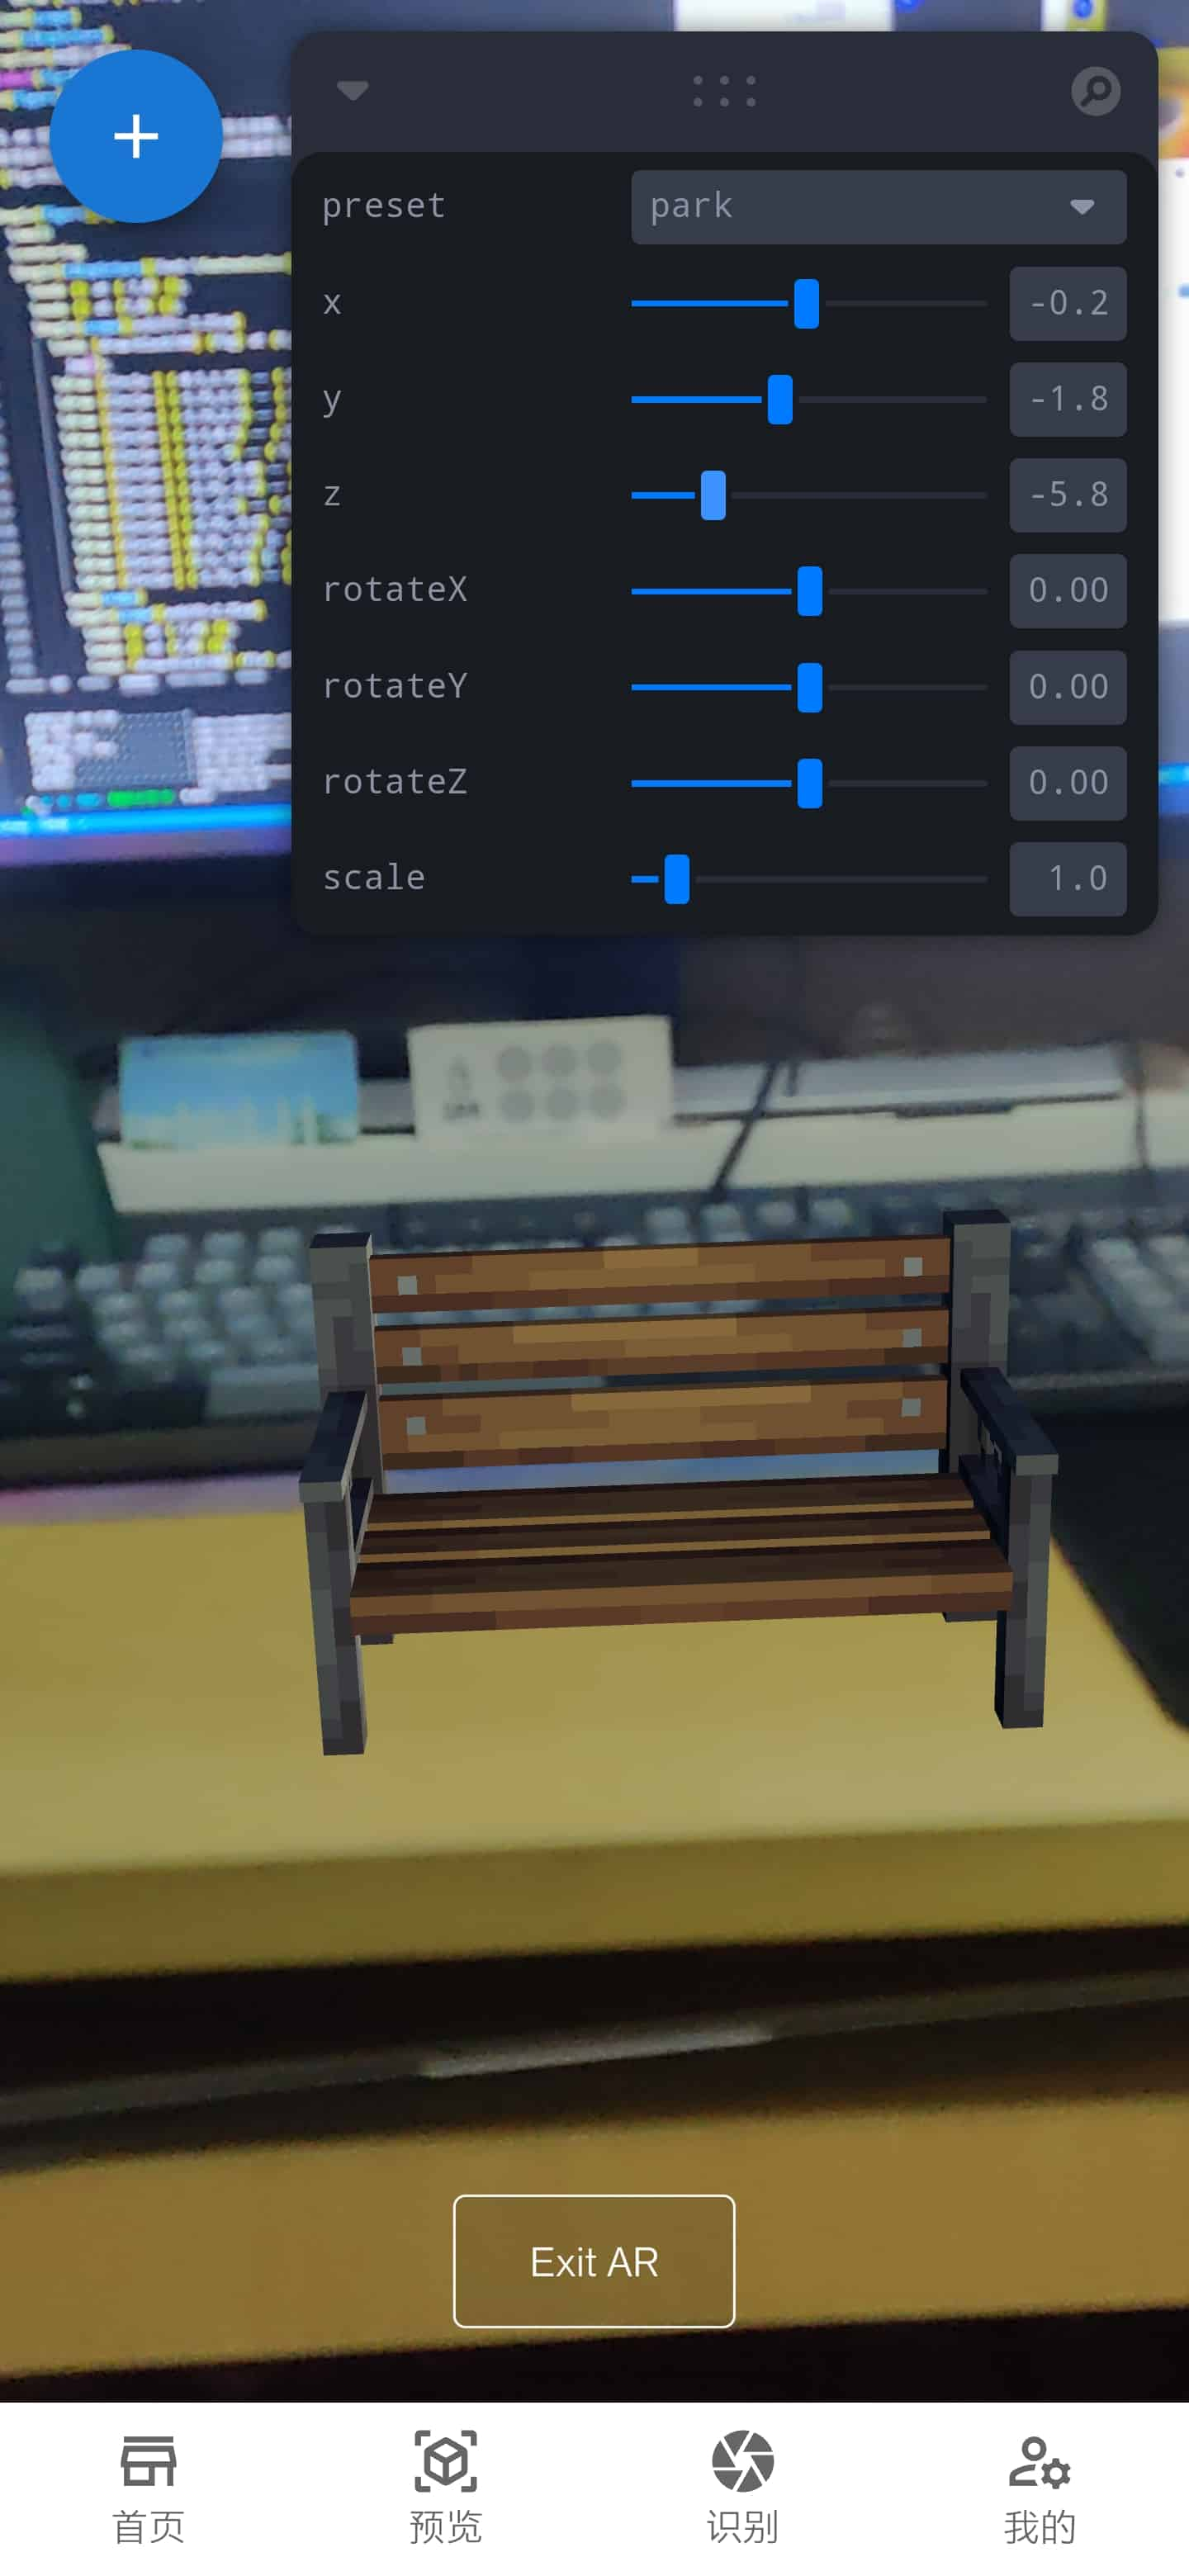
\includegraphics[width=4cm]{./figs/ar-preview-2.jpg}};
      \draw [Circle-] (1.75,3) -- (3,3) node [right] {设置模型位置参数};
      \draw [Circle-] (1.75,2) -- (3,2) node [right] {设置模型旋转参数};
      \draw [Circle-] (1.75,1.3) -- (3,1.3) node [right] {设置模型尺寸};
      \draw [Circle-] (-1.4,1) -- (3,1) node [right] {在 AR 模式中显示};
    \end{scope}
  \end{tikzpicture}
  \caption{AR预览界面}
  \label{fig:AR预览界面}
\end{figure}

进入 AR 识别界面后,系统首先会加载常规标记数据,如何通过设备地理位置在数据库中查找改区域内的标记加载。加载完所有标记数据后,系统实时匹配摄像机传输的图像,如果匹配上对应的标记,界面将弹出简略信息卡。AR 识别界面如图\ref{fig:AR识别界面}所示:

\begin{figure}[H]
  \small
  \centering
  \begin{tikzpicture}[font=\footnotesize]
    \node () at (-7,0) {};
    \node () at (7,0) {};
    \begin{scope}[xshift=-2.25cm]
      \node [draw=black!60] (fig) at (0,0) {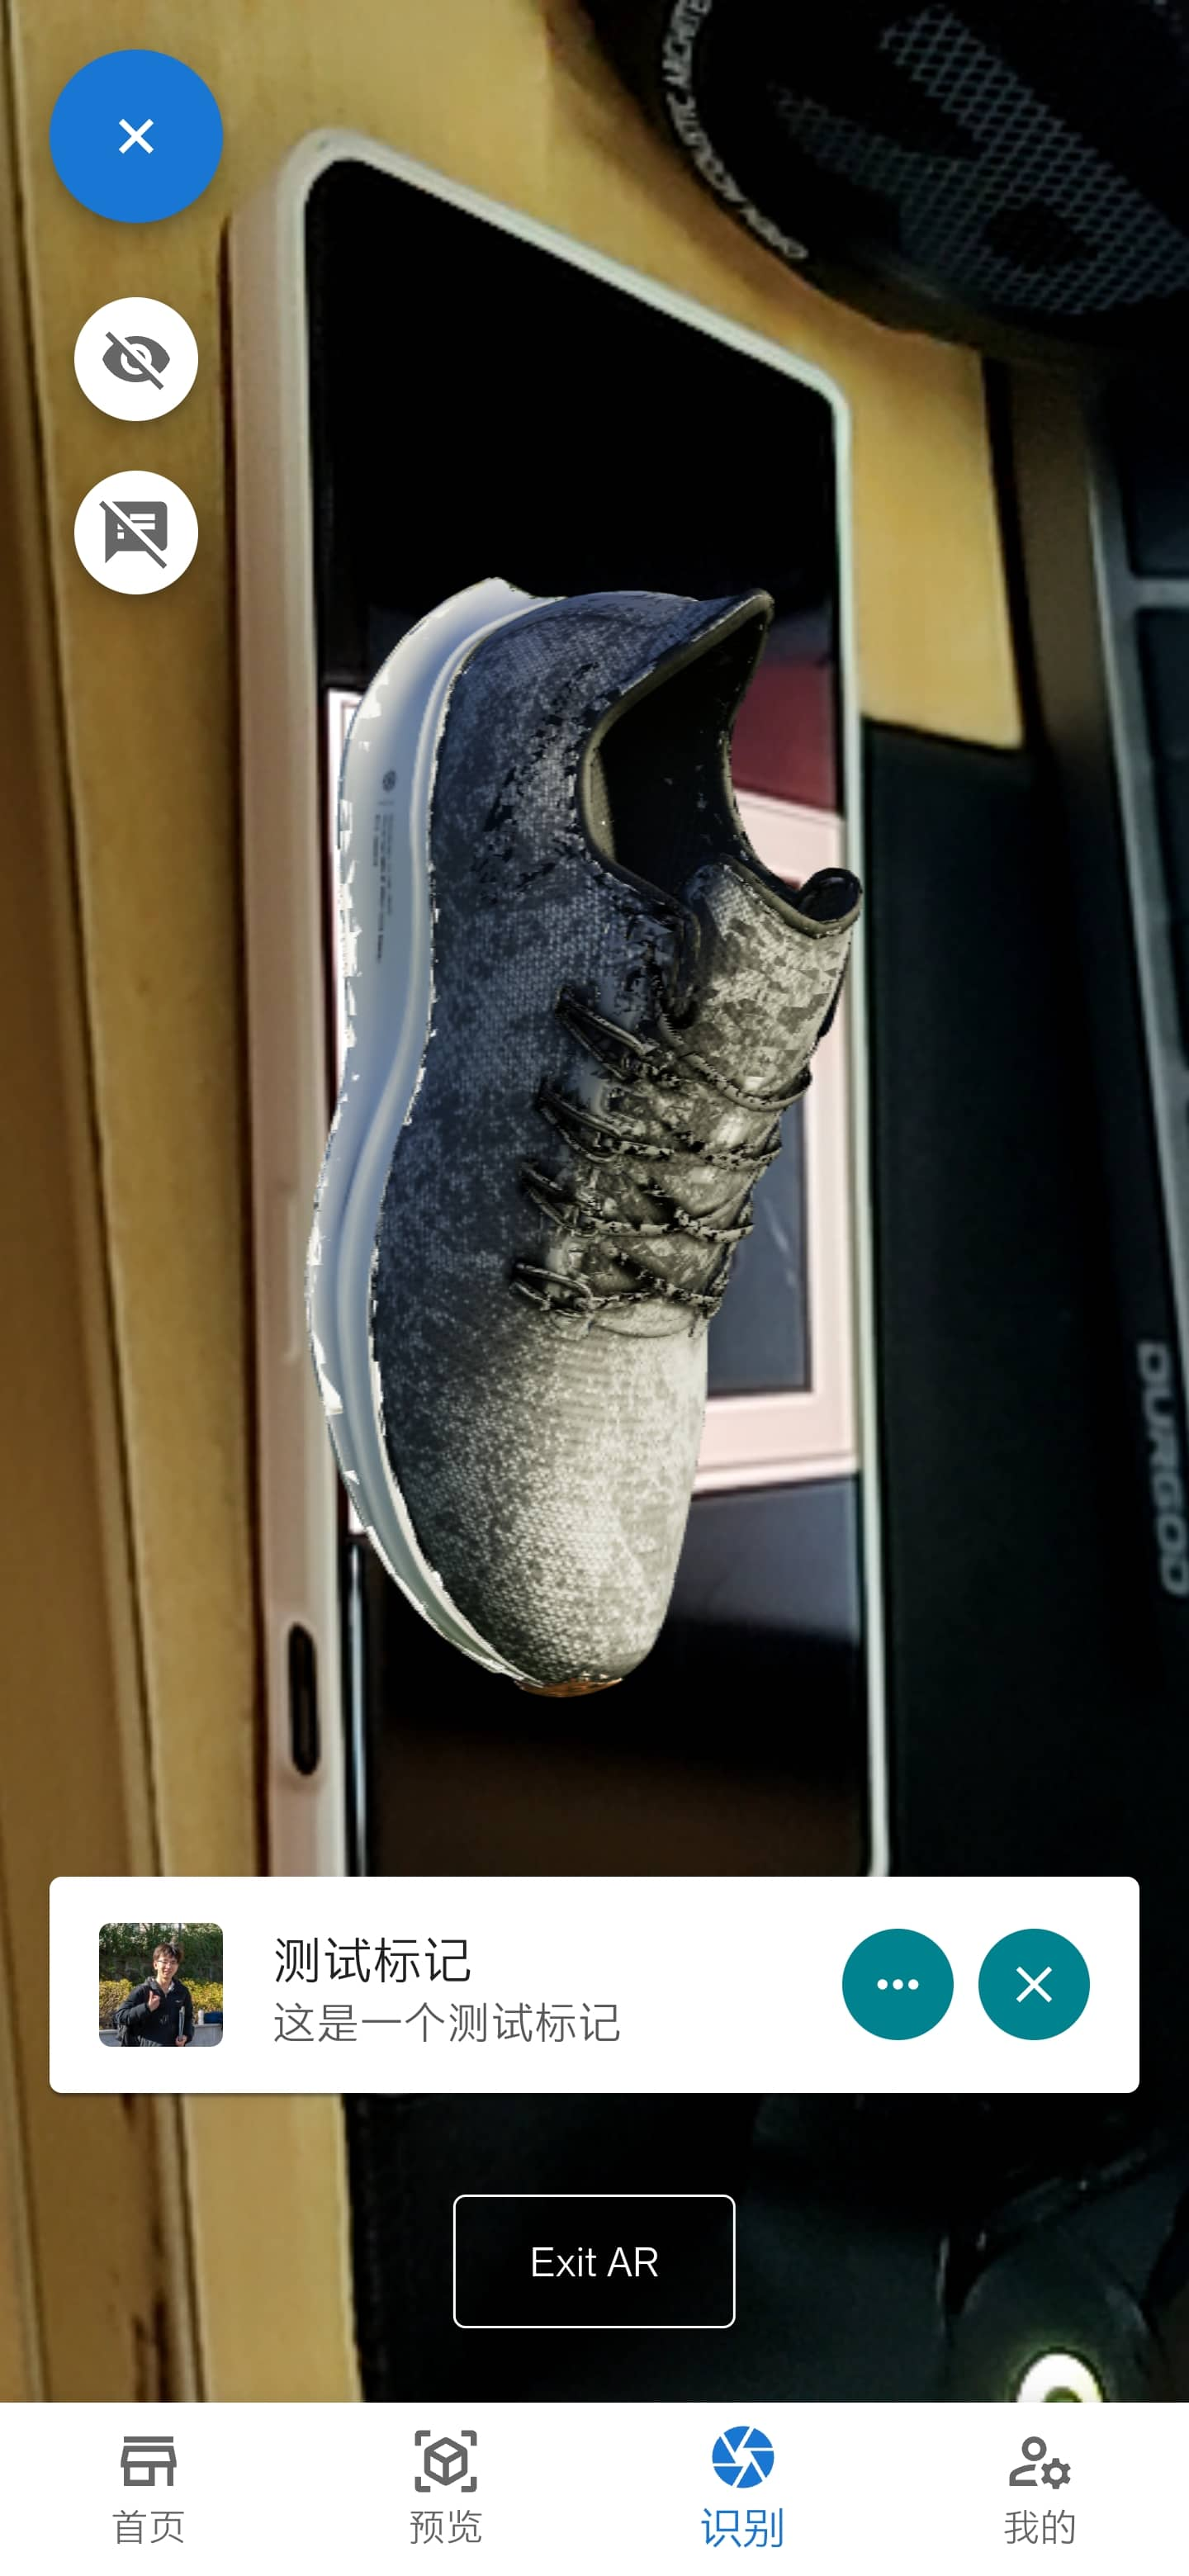
\includegraphics[width=4cm]{./figs/ar-identify.jpg}};
      \draw [Circle-] (-1.75,3.75) -- (-3,3.75) node [left] {扩展功能按钮};
      \draw [Circle-] (-1.75,3.1) -- (-3,3.1) node [left] {开关非必要组件};
      \draw [Circle-] (-1.75,2.5) -- (-3,2.5) node [left] {开关操作说明};
      \draw [Circle-] (0,0) -- (-3,0) node [left] {显示的模型};
      \draw [Circle-] (0.5,-0.5) -- (-3,-0.5) node [left] {匹配到的标记};
      \draw [Circle-] (-1.7,-2.3) -- (-3,-2.3) node [left] {标记简略信息卡};
      \draw [Circle-] (-0.25,-3.25) -- (-3,-3.25) node [left] {AR 按钮};
      \draw [Circle-] (-1.75,-4) -- (-3,-4) node [left] {其他模块链接};
    \end{scope}
    \begin{scope}[xshift=2.25cm]
      \node [draw=black!60] (fig) at (0,0) {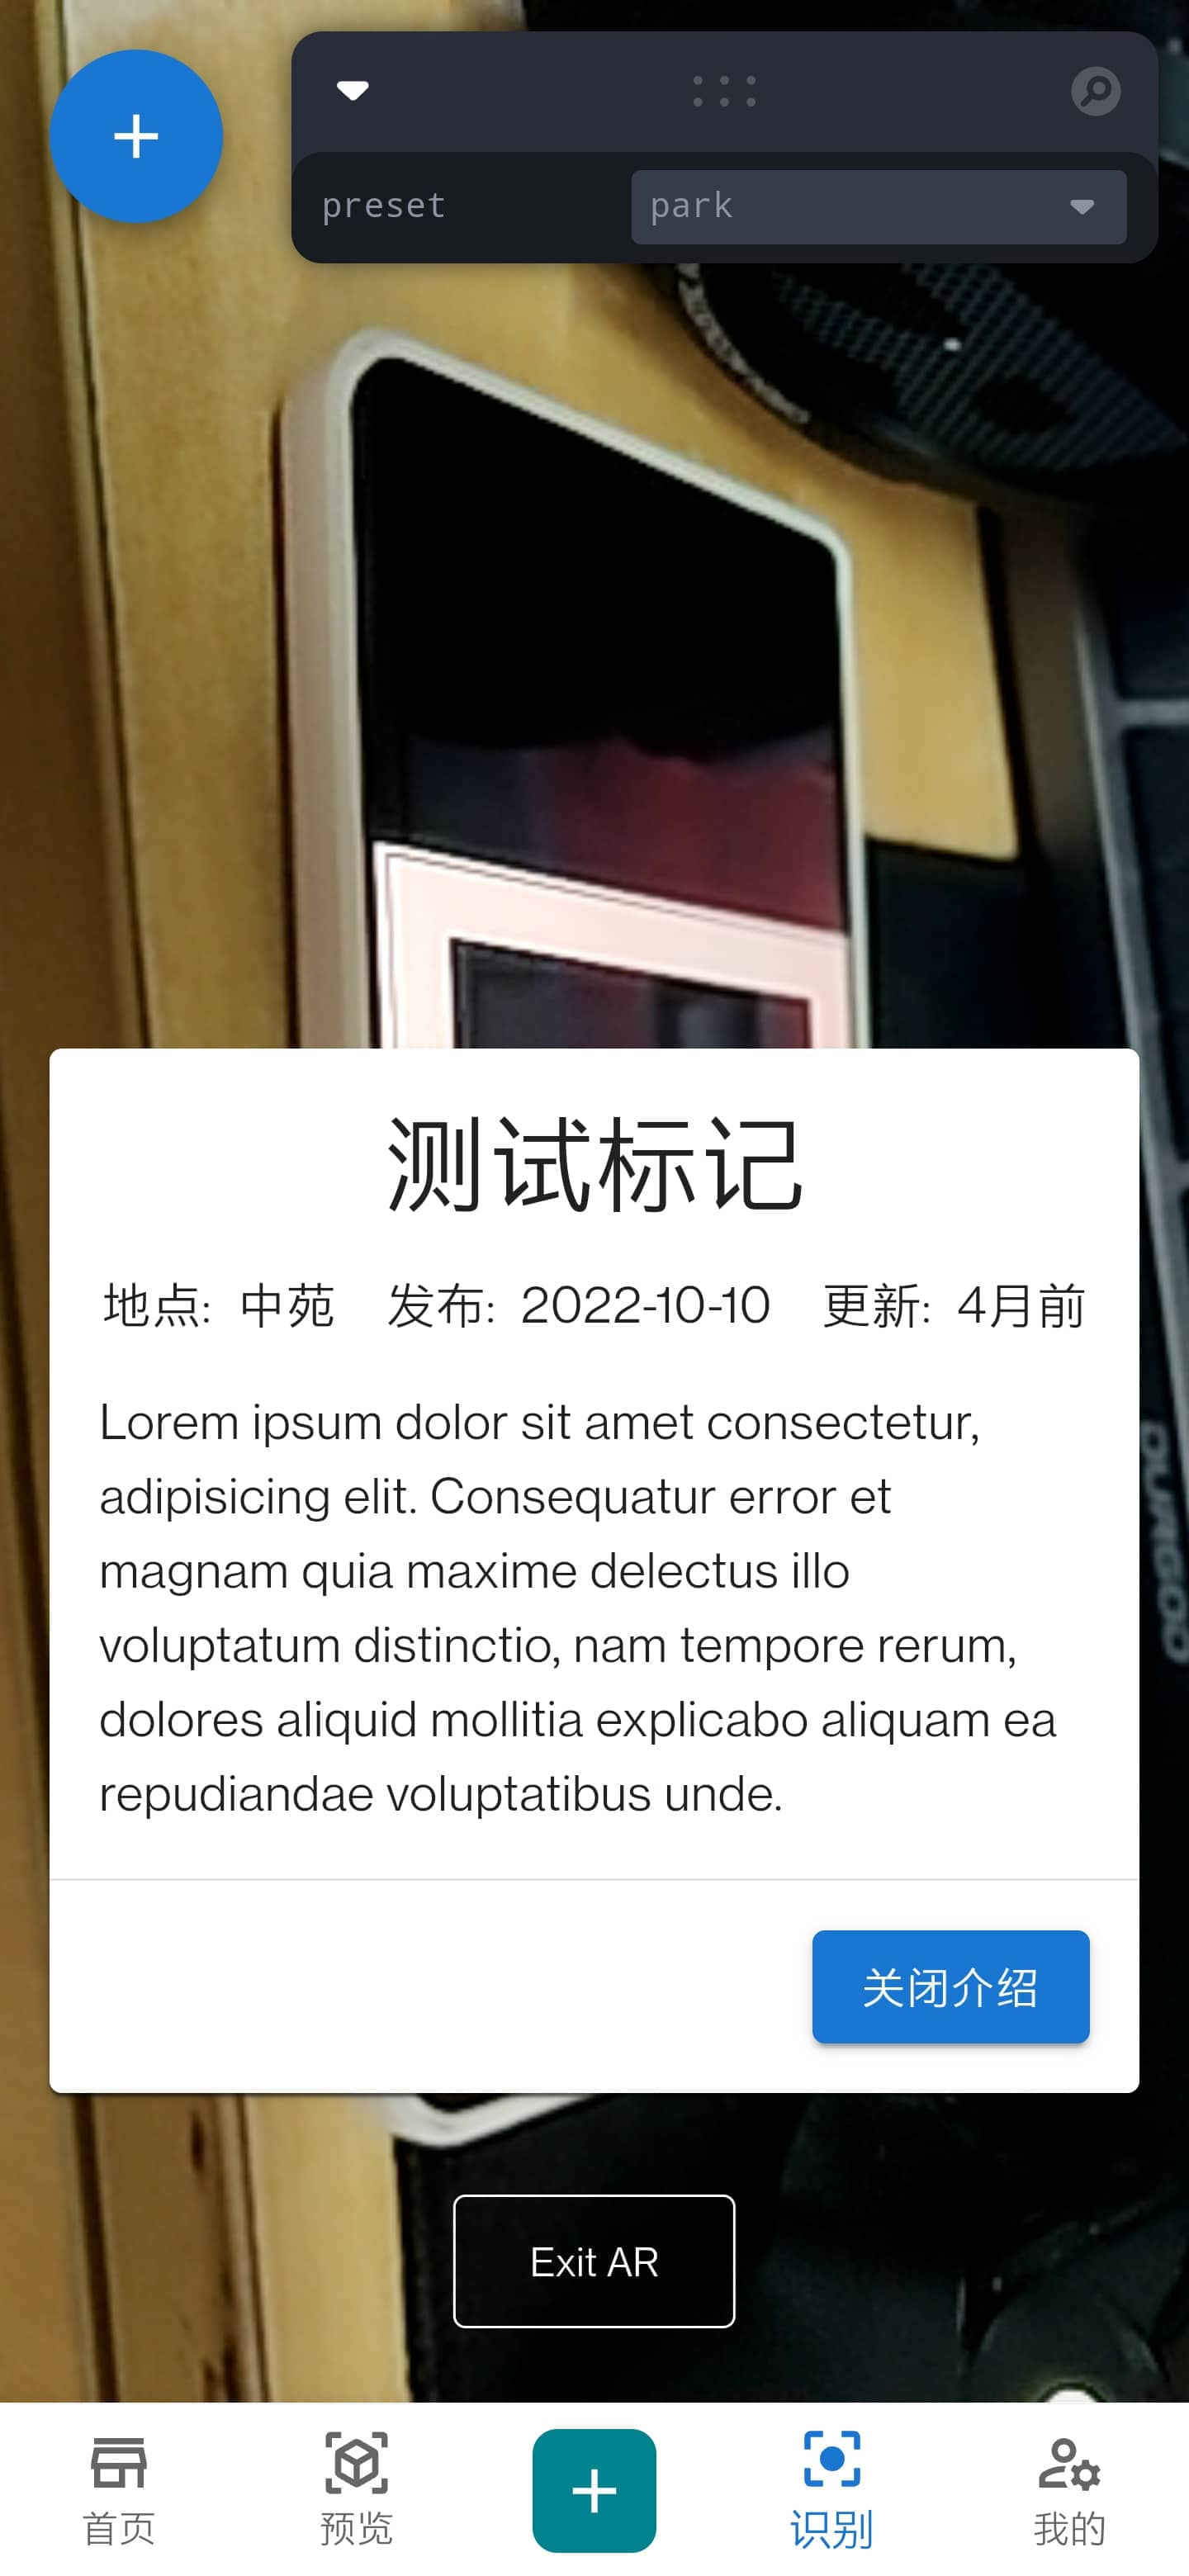
\includegraphics[width=4cm]{./figs/ar-identify-2.jpg}};
      \draw [Circle-] (0.5,4) -- (3,4) node [right] {控制板};
      \draw [Circle-] (1.75,3.6) -- (3,3.6) node [right] {设置模型背景};
      \draw [Circle-] (1.75,0) -- (3,0) node [right] {标记详细信息};
    \end{scope}
  \end{tikzpicture}
  \caption{AR识别界面}
  \label{fig:AR识别界面}
\end{figure}